\part{A Framework with the Serializability Guarantee}

\chapter{The \hemiola{} Domain-Specific Language}
\label{sec-hemiola-dsl}

As explained in \autoref{sec-sz-def}, on top of serializability, it is much easier to design and prove invariants.
That being said, it will still be a large burden if a user has to prove serializability per-protocol.
In this chapter, we would like to provide \emph{abstract conditions} to prove serializability, in order not to prove it directly for each protocol.
Furthermore, we design a domain-specific language (DSL) that every protocol defined on top of this language automatically satisfies the conditions to guarantee serializability.
The conditions have already been mentioned with the motivating example in \autoref{sec-nutshell} -- network topology and locking mechanisms, extracted from transient states of practical cache-coherence protocols.

\section{Topology and Network Requirements}
\label{sec-topo-net-reqs}

In order to employ the serializability guarantee in \hemiola{}, the objects in a given system should form a tree topology.
Most cache-coherent memory subsystems follow this topology, where leaf nodes correspond to L1 caches, and the root corresponds to the main memory.
A child and its parent in the tree communicate using the three channels shown in \autoref{sec-nutshell}: an upward-request channel, an upward-response channel, and a single downward channel.
Note that the use of the three channels does not mean the actual hardware implementation should use just the three channels; it can use any channel implementation that refines the three channels regarded as a specification.
For example, we may want to have an additional queue that accepts all the requests from child caches (from the corresponding upward-request channels), so the parent can have a single entry point to handle child requests.
We will indeed see in \autoref{sec-comp-syn} how logical channels in \hemiola{} are implemented at register-transfer level.

\hemiola{} as a Coq library generates the topology and network channels automatically from instances of a simple inductive type.
For example, the following tree definition will generate topology and channels for four L1 caches, two L2 caches, the last-level cache (LLC), and the main memory:
\begin{lstlisting}[numbers=none, frame=none]
  Definition t: tree := Node [Node [Node [Leaf; Leaf]; Node [Leaf; Leaf]]].
\end{lstlisting}

\section{Locking Mechanism}
\label{sec-locking-mechanism}

We saw in \autoref{sec-nutshell} why fine-grained transient states are required to ensure safe interleavings in cache-coherence protocols.
Revisiting the corner case described in \autoref{fig-motive-2}, a child should be able to handle an invalidation request from the parent even if it is in a transient state (SM), and after the response it changes its transient state to IM.
By looking at these transient states carefully, we have discovered that another necessary condition, other than the tree-topology condition, is the locking perspective from the transient states.

\hemiola{} supports a general locking mechanism reflecting this discovery;
instead of looking at the type of a message (\eg{} invalidation), the framework provides \emph{more-general} locking, just by looking at whether the message is from the parent or one of its children.
This relaxed locking mechanism is then not coupled with any specific cache-coherence protocols but is still sufficient to prove serializability.

\tikzset{
  uprightedge/.pic = {
    \draw [>->] (0.2, 0.25) -- (0.8, 1.05);
  },
}
\begin{figure}[h]
  \centering
  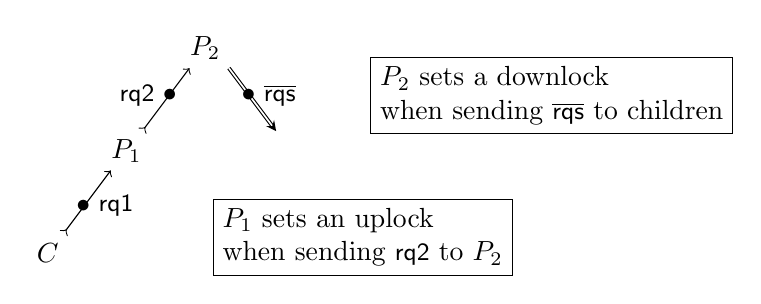
\begin{tikzpicture}
    \node at (0, 0) {$C$};
    \pic at (0, 0) {uprightedge};
    \node[label={[label distance=-4pt]right:{\small {\sf rq1}}}] at (0.45, 0.6) {$\bullet$};
    \node at (1.0, 1.3) {$P_1$};
    \pic at (1.0, 1.3) {uprightedge};
    \node[label={[label distance=-4pt]left:{\small {\sf rq2}}}] at (1.55, 2.0) {$\bullet$};
    \node at (2.0, 2.6) {$P_2$};

    \draw [>=stealth,double,->] (2.3, 2.35) -- (2.9, 1.55);
    \node[label={[label distance=-4pt]right:{\small $\overline{\textsf{rqs}}$}}] at (2.55, 2.0) {$\bullet$};

    \node[draw,align=left] at (4.0, 0.2) {$P_1$ sets an uplock\\ when sending {\small $\textsf{rq2}$} to $P_2$};
    \node[draw,align=left] at (6.4, 2.0) {$P_2$ sets a downlock\\ when sending {\small $\overline{\textsf{rqs}}$} to children};
  \end{tikzpicture}
  \caption{Locking mechanism in \hemiola{}}
  \label{fig-locking}
\end{figure}

In particular, \hemiola{} provides two kinds of locks: \emph{uplocks and downlocks}.
We say an object is uplocked (downlocked) when it holds an uplock (downlock).
\autoref{fig-locking} depicts the locking mechanism in \hemiola{}.
An uplock is set when an object makes an upward request to its parent ($P_1$ in the figure); it is released when the object gets a corresponding response from the parent.
On the contrary, a downlock is set when an object makes a downward request(s) to some of its children ($P_2$ in the figure).

\begin{figure}[h]
  \centering
  \renewcommand{\arraystretch}{1.2}
  \newcommand{\lockyes}{\cmark}
  \newcommand{\lockno}{\xmark}
  \begin{tabular}{ccc}
    \hline
    & Uplocked & Downlocked\\
    \hline
    Acquiring an uplock & \lockno & \lockyes\\
    Releasing an uplock & \lockyes & \lockno\\
    Acquiring a downlock & \lockyes & \lockno\\
    Releasing a downlock & \lockyes & \lockyes\\
    \hline
  \end{tabular}
  \caption{Locking conditions in \hemiola{}}
  \label{fig-locking-conditions}
\end{figure}

\autoref{fig-locking-conditions} shows the conditions to acquire or release the locks.
An uplock can be set if the object is not yet uplocked; it can be set even when the object is downlocked.
This locking mechanism means that an object can make a request to the parent even when it has made requests to the children.
It is still safe, since the lock release will not be allowed when downlocked, \ie{} the uplock release should always wait for the downlock to be released.
On the other hand, a downlock \emph{can be set and released even when uplocked}.
This relaxation is very important to make the locking mechanism both safe and live.
If a downlock could not be released when uplocked, we would have a deadlock case, where both locks wait for each other.

Now every cache object defined in \hemiola{} \emph{does not need to set transient states} to consider all combinations among stable statuses;
instead, the framework helps maintain the cache status and claim proper locks.
For example, instead of setting a transient state SM, it is now desirable to maintain its status S and to set an uplock to record it just made the upward request.
(The framework provides even more, actually, by guiding users to employ the \emph{rule templates}, introduced in the next section, that automatically set proper locks.)

Each object defined in \hemiola{} has a semantic \emph{lock state}, a finite map from a lock type (uplock or downlock) to lock information: the original request message, the original requestor index, and requestee indices from which we expect to get responses.
In the common terminology of cache-coherence protocols, each lock corresponds to a miss status holding register (MSHR).
An MSHR is set when a cache miss happens and the miss triggers further requests to obtain a proper status and up-to-date data.
As with \hemiola{} lock holders, MSHRs play a crucial role both in deciding whether to handle certain requests and in storing information needed to handle them properly.

It is worth emphasizing that an uplock and a downlock are assigned for each line.
In other words, the locking conditions presented in \autoref{fig-locking-conditions} do not apply to the locks for different cache lines.
This separation is safe, since in a cache-coherence protocol the transactions for different cache lines never interfere with each others.
It is not practical, however, to have an uplock and a downlock for each line in the actual hardware implementation.
We need to restrict the number of locks (MSHRs) to make the implementation synthesizable.
A detailed discussion about this restriction will be provided in \autoref{sec-comp-syn}.

\section{Rule Templates}
\label{sec-rule-templates}

\newcommand{\rtname}[1]{{\small\sf\bf #1}}

\newcommand{\uled}{\ensuremath{\textsf{UL}}}
\newcommand{\dled}{\ensuremath{\textsf{DL}}}
\newcommand{\ulfree}{\ensuremath{\textsf{UL}_{\times}}}
\newcommand{\dlfree}{\ensuremath{\textsf{DL}_{\times}}}

\newcommand{\setul}{\ensuremath{\textsf{UL}\Uparrow}}
\newcommand{\setdl}{\ensuremath{\textsf{DL}\Uparrow}}
\newcommand{\relul}{\ensuremath{\textsf{UL}\Downarrow}}
\newcommand{\reldl}{\ensuremath{\textsf{DL}\Downarrow}}
\newcommand{\stsilent}{\ensuremath{\textsf{SLT}}}

\newcommand{\ppo}[3]{\ensuremath{\{#1\}#2\lbrack#3\rbrack}}
\newcommand*{\bfrac}[2]{\genfrac{}{}{0pt}{}{#1}{#2}}

On top of the topology/network requirements and the locking mechanism, \hemiola{} provides rule templates to ensure that objects communicate within the topology and locks are properly set.
In this section, we will explore what kinds of rule templates \hemiola{} provides and discuss their uses.
Each rule template will be introduced with the form $\ppo{P}{O}{Q}$ and arrows with $\circ$ and $\bullet$, which means that the rule template is for an object $O$, requires input messages ($\circ$) and a precondition $P$, performs a state transition $Q$, and generates output messages ($\bullet$).
$\uled$, $\dled$, $\ulfree$, and $\dlfree$ in a precondition indicate that the object is uplocked, downlocked, uplock-free, and downlock-free, respectively.
$\setul$, $\setdl$, $\relul$, and $\reldl$ in a state transition indicate setting an uplock, setting a downlock, releasing an uplock, and releasing a downlock, respectively.
$\stsilent{}$ annotates that the rule template forbids any state modification beside locking.

\paragraph{Rule templates for immediate responses}

\begin{center}
  \begin{tabular}{p{0.18\textwidth}p{0.77\textwidth}}
    \begin{adjustbox}{valign=t}
      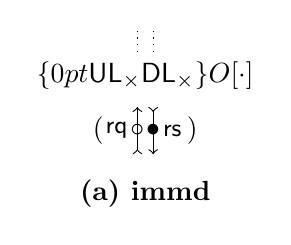
\begin{tikzpicture}
        \draw [dotted] (-0.1, 0.5) -- (-0.1, 0.8);
        \draw [dotted] (0.1, 0.5) -- (0.1, 0.8);
        \node at (0, 0.2) {$\ppo{\bfrac{\ulfree{}}{\dlfree{}}}{O}{\cdot}$};
        \draw [<-<] (-0.1, -0.2) -- (-0.1, -0.8);
        \draw [>->] (0.1, -0.2) -- (0.1, -0.8);
        \node[label={[label distance=-6pt]left:{\small {\sf rq}}}] at (-0.1, -0.5) {$\circ$};
        \node[label={[label distance=-6pt]right:{\small {\sf rs}}}] at (0.1, -0.5) {$\bullet$};
        \node at (0, -0.5) {$(\qquad\quad)$};
        \node at (0, -1.3) {{\bf (a) immd}};
      \end{tikzpicture}
    \end{adjustbox}&
    An immediate-down ({\bf immd}) rule responds immediately to an upward request, requiring both locks be free.
    This rule allows not to take (generate) any input (output) messages.
    (The input/output messages are parenthesized in the form.)
    In other words, using this rule, an object can make a local state transition without any input/output messages, but in this case both locks should be free.
    This rule also shows that a transaction may start without any input messages as a trigger, which still matches the definition of externally atomic histories in \autoref{fig-atomic-trs}.
  \end{tabular}
\end{center}

\begin{center}
  \begin{tabular}{p{0.18\textwidth}p{0.77\textwidth}}
    \begin{adjustbox}{valign=t}
      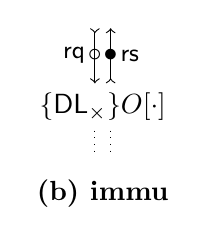
\begin{tikzpicture}
        \draw [<-<] (-0.1, 0.1) -- (-0.1, 0.8);
        \draw [>->] (0.1, 0.1) -- (0.1, 0.8);
        \node at (0, -0.2) {$\ppo{\dlfree{}}{O}{\cdot}$};
        \draw [dotted] (-0.1, -0.5) -- (-0.1, -0.8);
        \draw [dotted] (0.1, -0.5) -- (0.1, -0.8);
        \node[label={[label distance=-6pt]left:{\small {\sf rq}}}] at (-0.1, 0.45) {$\circ$};
        \node[label={[label distance=-6pt]right:{\small {\sf rs}}}] at (0.1, 0.45) {$\bullet$};
        \node at (0, -1.3) {{\bf (b) immu}};
      \end{tikzpicture}
    \end{adjustbox}&
    An immediate-up ({\bf immu}) rule responds immediately to a downward request, and it only requires the downlock be free.
    In other words, even when uplocked, an object can make a state transition by taking a downward request and generating an upward response immediately.\\
  \end{tabular}
\end{center}

\paragraph{Rule templates to communicate with the parent}

\begin{center}
  \begin{tabular}{p{0.18\textwidth}p{0.77\textwidth}}
    \begin{adjustbox}{valign=t}
      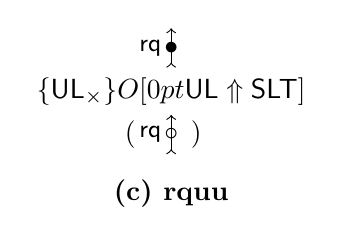
\begin{tikzpicture}
        \draw [>->] (0, 0.3) -- (0, 0.8);
        \node at (0, 0) {$\ppo{\ulfree{}}{O}{\bfrac{\setul{}}{\stsilent{}}}$};
        \draw [<-<] (0, -0.3) -- (0, -0.8);
        \node[label={[label distance=-6pt]left:{\small {\sf rq}}}] at (0, -0.55) {$\circ$};
        \node[label={[label distance=-6pt]left:{\small {\sf rq}}}] at (0, 0.55) {$\bullet$};
        \node at (-0.1, -0.55) {$(\qquad)$};
        \node at (0, -1.3) {{\bf (c) rquu}};
      \end{tikzpicture}
    \end{adjustbox}&
    A request-up-up ({\bf rquu}) rule (possibly) takes an upward request from a child and make another request to the parent.
    It requires the uplock to be free but does not care whether the object is downlocked or not.
    A state transition is not allowed when setting any lock (either an uplock or a downlock).
  \end{tabular}
\end{center}

\begin{center}
  \begin{tabular}{p{0.18\textwidth}p{0.77\textwidth}}
    \begin{adjustbox}{valign=t}
      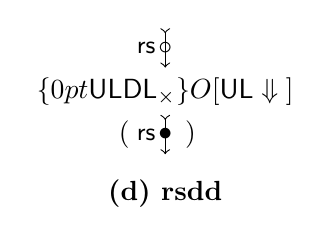
\begin{tikzpicture}
        \draw [<-<] (0, 0.3) -- (0, 0.8);
        \node at (0, 0) {$\ppo{\bfrac{\uled{}}{\dlfree{}}}{O}{\relul{}}$};
        \draw [>->] (0, -0.3) -- (0, -0.8);
        \node[label={[label distance=-6pt]left:{\small {\sf rs}}}] at (0, 0.55) {$\circ$};
        \node[label={[label distance=-6pt]left:{\small {\sf rs}}}] at (0, -0.55) {$\bullet$};
        \node at (-0.1, -0.55) {$(\qquad)$};
        \node at (0, -1.3) {{\bf (d) rsdd}};
      \end{tikzpicture}
    \end{adjustbox}&
    A response-down-down ({\bf rsdd}) rule is dual to the {\bf rquu} rule, which takes a downward response and (possibly) responds to the original child requestor.
    This rule releases the corresponding uplock.
    Note that in order to handle a response from the parent, the object should be downlock-free.
    This precondition is indeed required to ensure correctness (serializability), as explained in \autoref{sec-locking-mechanism}.
  \end{tabular}
\end{center}

\paragraph{Rule templates to communicate with children}

\begin{center}
  \begin{tabular}{p{0.18\textwidth}p{0.77\textwidth}}
    \begin{adjustbox}{valign=t}
      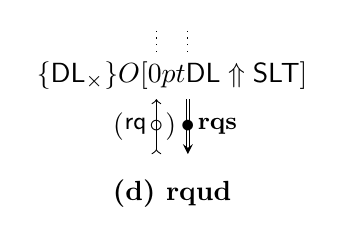
\begin{tikzpicture}
        \draw [dotted] (-0.2, 0.5) -- (-0.2, 0.8);
        \draw [dotted] (0.2, 0.5) -- (0.2, 0.8);
        \node at (0, 0.2) {$\ppo{\dlfree{}}{O}{\bfrac{\setdl{}}{\stsilent{}}}$};
        \draw [<-<] (-0.2, -0.1) -- (-0.2, -0.8);
        \draw [>=stealth,double,->] (0.2, -0.1) -- (0.2, -0.8);
        \node[label={[label distance=-6pt]left:{\small {\sf rq}}}] at (-0.2, -0.45) {$\circ$};
        \node[label={[label distance=-6pt]right:{\small {\sf {\bf rqs}}}}] at (0.2, -0.45) {$\bullet$};
        \node at (-0.35, -0.45) {$(\enspace\quad)$};
        \node at (0, -1.3) {{\bf (d) rqud}};
      \end{tikzpicture}
    \end{adjustbox}&
    A request-up-down ({\bf rqud}) rule (possibly) takes an upward request and makes downward requests to some of the children except the child requestor.
    A downlock is set in this case, and thus no state transition is allowed.
    This rule does not have a precondition that the object should be uplock-free, \ie{} the object can handle a request from the parent even when uplocked.
    This relaxation is still safe in terms of correctness (serializability) and necessary to avoid a deadlock.
  \end{tabular}
\end{center}

\begin{center}
  \begin{tabular}{p{0.18\textwidth}p{0.77\textwidth}}
    \begin{adjustbox}{valign=t}
      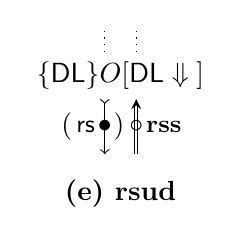
\begin{tikzpicture}
        \draw [dotted] (-0.2, 0.5) -- (-0.2, 0.8);
        \draw [dotted] (0.2, 0.5) -- (0.2, 0.8);
        \node at (0, 0.2) {$\ppo{\dled{}}{O}{\reldl{}}$};
        \draw [>->] (-0.2, -0.1) -- (-0.2, -0.8);
        \draw [>=stealth,double,<-] (0.2, -0.1) -- (0.2, -0.8);
        \node[label={[label distance=-6pt]left:{\small {\sf rs}}}] at (-0.2, -0.45) {$\bullet$};
        \node[label={[label distance=-6pt]right:{\small {\sf {\bf rss}}}}] at (0.2, -0.45) {$\circ$};
        \node at (-0.35, -0.45) {$(\enspace\quad)$};
        \node at (0, -1.3) {{\bf (e) rsud}};
      \end{tikzpicture}
    \end{adjustbox}&
    A response-up-down ({\bf rsud}) rule is dual to the {\bf rqud} rule, which takes upward responses and (possibly) responds back to the original child requestor.
    The rule releases the corresponding downlock.
    As explained in \autoref{sec-locking-mechanism}, it does not require any conditions on the uplock.
  \end{tabular}
\end{center}

\begin{center}
  \begin{tabular}{p{0.18\textwidth}p{0.77\textwidth}}
    \begin{adjustbox}{valign=t}
      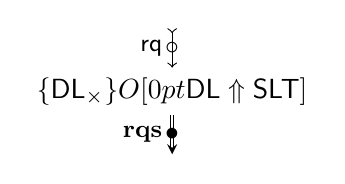
\begin{tikzpicture}
        \draw [<-<] (0, 0.3) -- (0, 0.8);
        \node at (0, 0) {$\ppo{\dlfree{}}{O}{\bfrac{\setdl{}}{\stsilent{}}}$};
        \draw [>=stealth,double,->] (0, -0.3) -- (0, -0.8);
        \node[label={[label distance=-6pt]left:{\small {\sf rq}}}] at (0, 0.55) {$\circ$};
        \node[label={[label distance=-6pt]left:{\small {\sf {\bf rqs}}}}] at (0, -0.55) {$\bullet$};
      \end{tikzpicture}
    \end{adjustbox}&
    A request-down-down ({\bf rqdd}) rule takes a downward request (from the parent) and makes downward requests to some of the children.
    Similar to {\bf rqud}, a downlock is set, and no state transition is allowed.
    This rule also does not require the object to be uplock-free, which is to avoid a deadlock.
  \end{tabular}
\end{center}

\begin{center}
  \begin{tabular}{p{0.18\textwidth}p{0.77\textwidth}}
    \begin{adjustbox}{valign=t}
      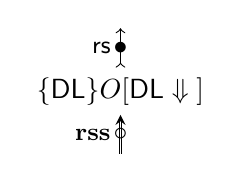
\begin{tikzpicture}
        \draw [>->] (0, 0.3) -- (0, 0.8);
        \node at (0, 0) {$\ppo{\dled{}}{O}{\reldl{}}$};
        \draw [>=stealth,double,<-] (0, -0.3) -- (0, -0.8);
        \node[label={[label distance=-6pt]left:{\small {\sf rs}}}] at (0, 0.55) {$\bullet$};
        \node[label={[label distance=-6pt]left:{\small {\sf {\bf rss}}}}] at (0, -0.55) {$\circ$};
      \end{tikzpicture}
    \end{adjustbox}&
    A response-up-up ({\bf rsuu}) rule is dual to the {\bf rqdd} rule, which takes upward responses and responds back to the parent.
    Similar to {\bf rsud}, this rule also releases the corresponding downlock.
  \end{tabular}
\end{center}

\paragraph{A rule template for whole-tree traversal}

\begin{center}
  \begin{tabular}{p{0.18\textwidth}p{0.77\textwidth}}
    \begin{adjustbox}{valign=t}
      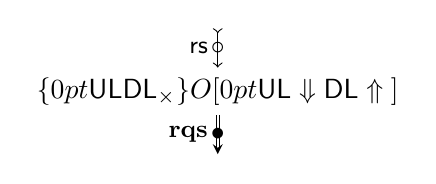
\begin{tikzpicture}
        \draw [<-<] (0, 0.3) -- (0, 0.8);
        \node at (0, 0) {$\ppo{\bfrac{\uled{}}{\dlfree{}}}{O}{\bfrac{\relul{}}{\setdl{}}}$};
        \draw [>=stealth,double,->] (0, -0.3) -- (0, -0.8);
        \node[label={[label distance=-6pt]left:{\small {\sf rs}}}] at (0, 0.55) {$\circ$};
        \node[label={[label distance=-6pt]left:{\small {\sf {\bf rqs}}}}] at (0, -0.55) {$\bullet$};
      \end{tikzpicture}
    \end{adjustbox}&
    A response-down-request-down rule ({\bf rsrq}) takes a downward response (from the parent) and makes new downward requests to some of the children.
    It makes a \emph{transfer} from an uplock to a new downlock by releasing the uplock and setting a downlock, where the child-requestor information is moved from the uplock.
    This rule forces the order of a traversal, saying that the traversal for the outer objects must be done before traversing the inner objects.
    The forced order is important to avoid a deadlock.
    For example, if the object makes requests to its parent and children at the same time and sets both an uplock and a downlock, a deadlock may occur.
  \end{tabular}
\end{center}

\paragraph{Remarks}

The rule templates are designed carefully to perform any practical transactions \emph{safely} with serializable behavior.
Consider an extreme case in a cache-coherence protocol.
When an L1 cache wants to obtain a write permission, all the other caches should be invalidated (changing each cache status to Invalid).
In order to perform such a transaction, it must be able to traverse all the other caches.
This transaction kind is one of the longest-running in cache-coherence protocols, and the rule templates are designed with proper locking ($\uled$ and $\dled$) and a state-change condition ($\stsilent$), not to create any incoherence while such a long transaction is interleaved with other transactions.

\chapter{Serializability Guarantee by \hemiola{}}

In this chapter, we provide the proof of serializability in \hemiola{}.
As introduced in \autoref{sec-hemiola-dsl}, the proof largely requires the two conditions: the tree topology with the three channel kinds (introduced in \autoref{sec-topo-net-reqs}) and the locking mechanism (introduced in \autoref{sec-locking-mechanism}).
Since the \hemiola{} DSL with the rule templates faithfully follows such conditions, we can also say that just using the DSL ensures serializability.
While conventional approaches to verifying cache-coherence protocols deal with transient states directly and induce noninterference lemmas per-state, \hemiola{} provides the serializability guarantee as \emph{the most general form of noninterference, obtained from conditions that are not coupled to any specific cache-coherence protocol}, \eg{} the DSL does not mention anything about cache-coherence protocols.

In proving serializability we use a well-established technique called commuting reductions~\cite{reduction}.
This reduction technique has been used before to prove correctness of concurrent software~\cite{Chajed:2018} and distributed systems~\cite{Hawblitzel:2015,Hawblitzel:2017}, but to our knowledge no past work has tried to discover serializability conditions for cache-coherence protocols and proved them using reductions.

\section{The Intuition: Merging Atomic-History Fragments}
\label{sec-sz-pf-intuition}

\newcommand{\commstep}[2]{\ensuremath{#1 \leftrightarrowtriangle #2}}
\newcommand{\commhst}[2]{\ensuremath{#1 \leftrightarrowtriangle #2}}

We first present our intuition of how commuting reductions are used in the serializability proof; in order for it, we need to formalize commuting reductions first.
The most basic commuting reduction happens between two adjacent state-transition steps:
\begin{definition}[Commutativity of steps]
  \label{def-comm-steps}
  Two adjacent state-transition steps commute, denoted as \commstep{(\semstep{S}{s_0}{l_0}{s_1})}{(\semstep{S}{s_1}{l_1}{s_2})}, if the state transitions with the opposite order reach the same state:
  \begin{displaymath}
    \commstep{(\semstep{S}{s_0}{l_0}{s_1})}{(\semstep{S}{s_1}{l_1}{s_2})} \triangleq \exists s_1'.\; \semstep{S}{s_0}{l_1}{s_1'} \wedge \semstep{S}{s_1'}{l_0}{s_2}.
  \end{displaymath}
\end{definition}
We will write just $\commstep{l_0}{l_1}$ when the system $S$ and the transition-step adjacency (\ie{} existence of the intermediate state $s_1$) are clear from context.

We can naturally lift the definition to one for histories to argue whether two histories commute or not:
\begin{definition}[Commutativity of histories]
  \label{def-comm-hsts}
  Two adjacent histories commute, denoted as \commstep{(\semsteps{S}{s_0}{h_0}{s_1})}{(\semstep{S}{s_1}{h_1}{s_2})}, if the state transitions with the opposite order reach the same state:
  \begin{displaymath}
    \commhst{(\semsteps{S}{s_0}{h_0}{s_1})}{(\semsteps{S}{s_1}{h_1}{s_2})} \triangleq \exists s_1'.\; \semsteps{S}{s_0}{h_1}{s_1'} \wedge \semsteps{S}{s_1'}{h_0}{s_2}.
  \end{displaymath}
\end{definition}
We overload the same notation for history commutativity.
We will also use the shorter version $\commhst{h_0}{h_1}$ with clear context.

Our high-level intuition for the serializability proof is that for a given interleaved history we can perform a finite number of reductions to get a sequential history that reaches the same state.
More specifically, we will try to \emph{merge} any two separated atomic-history fragments by performing reductions.

\begin{figure}[t]
  \centering
  \begin{tabular}{cc}
    \begin{tikzpicture}
      \pic at (0, 0) {skeleton-pcce1={$P$}{$C_1$}{$C_2$}};
      % C_1 external
      \pic at (0, 0) {skeleton-midx-e1};
      \node[label={[label distance=-6pt,myred]left:{\small {\sf rqWr}}},color=myred] at (-1.8, -2.3) {$\bullet$};
      \node[label={[label distance=-6pt,myred]right:{\small {\sf rsWr}}},color=myred] at (-1.6, -2.3) {$\bullet$};
      % Between P and C_1
      \pic at (0, 0) {skeleton-midx-pc1};
      \node[label={[label distance=-6pt,myred]left:{\small {\sf rqM}}},color=myred] at (-1, -0.7) {$\bullet$};
      \node[label={[label distance=-9pt,myred]below right:{\small {\sf rsM}}},color=myred] at (-0.6, -0.7) {$\bullet$};
      % Between P and C_2
      \pic at (0, 0) {skeleton-midx-pc2};
      \node[label={[label distance=-9pt,myred]below left:{\small {\sf rsI}}},color=myred] at (0.8, -0.7) {$\bullet$};
      \node[label={[label distance=-6pt,myred]right:{\small {\sf rqI}}},color=myred] at (1, -0.7) {$\bullet$};

      % Curves
      \draw [->,color=myred] (-2.3, -2.0) to[out=90,in=-90] node[left] {\rdcircflsm{1}{rquu}} (-1.8, -1.0);
      \draw [->,color=myred] (-1.7, -0.4) to[out=70,in=110,distance=1.8cm] node[left=18pt] {\rdcircflsm{3}{rqud}} (1.4, -0.4);
      \draw [->,color=myred] (1.6, -0.9) to[out=-50,in=-50,distance=1.9cm] node[below] {\rdcircflsm{4}{immu}} (0.5, -1.3);
      \draw [->,color=myred] (0.4, -0.8) to[out=135,in=45,distance=0.6cm] (-0.3, -0.7);
      \draw [densely dashed,color=myred,line width=0.3pt] (0, -0.35) to[out=90,in=-170] (1.6, 0.35);
      \node at (2.0, 0.3) {\rdcircflsm{5}{rsud}};
      \draw [->,color=myred] (-0.6, -1.1) to[out=225,in=90] node[below right] {\rdcircflsm{7}{rsdd}} (-1.1, -2.0);
    \end{tikzpicture} &
    \begin{tikzpicture}
      \pic at (0, 0) {skeleton-pcce2={$P$}{$C_1$}{$C_2$}};
      % C_2 external
      \pic at (0, 0) {skeleton-midx-e2};
      \node[label={[label distance=-6pt,myblue]right:{\small {\sf rsWr}}},color=myblue] at (1.8, -2.3) {$\bullet$};
      \node[label={[label distance=-6pt,myblue]left:{\small {\sf rqWr}}},color=myblue] at (1.6, -2.3) {$\bullet$};
      % Between P and C_1
      \pic at (0, 0) {skeleton-midx-pc1};
      \node[label={[label distance=-9pt,myblue]above left:{\small {\sf rsI}}},color=myblue] at (-0.8, -0.7) {$\bullet$};
      \node[label={[label distance=-10pt,myblue]below right:{\small {\sf rqI}}},color=myblue] at (-0.6, -0.7) {$\bullet$};
      % Between P and C_2
      \pic at (0, 0) {skeleton-midx-pc2};
      \node[label={[label distance=-6pt,myblue]right:{\small {\sf rsM}}},color=myblue] at (1, -0.7) {$\bullet$};
      \node[label={[label distance=-6pt,myblue]below:{\small {\sf rqM}}},color=myblue] at (0.6, -0.7) {$\bullet$};

      % Curves
      \draw [->,color=myblue] (1.1, -2.0) to[out=90,in=-45] node[below left=-3pt] {\blcircflsm{2}{rquu}} (0.6, -1.3);
      \draw [->,color=myblue] (0.4, -0.8) to[out=135,in=45,distance=0.5cm] (-0.3, -0.7);
      \draw [densely dashed,color=myblue,line width=0.3pt] (0, -0.35) to[out=90,in=-170] (1.6, 0.35);
      \node at (2.0, 0.3) {\blcircflsm{6}{rqud}};
      \draw [->,color=myblue] (-0.6, -1.2) to[out=-135,in=-135,distance=2.1cm] node[below] {\blcircflsm{8}{immu}} (-1.4, -0.7);
      \draw [->,color=myblue] (-1.1, -0.2) to[out=60,in=120,distance=1.7cm] node[left=18pt] {\blcircflsm{9}{rsud}} (1.4, -0.5);
      \draw [->,color=myblue] (1.7, -0.95) to[out=-90,in=90] node[above right=-2pt] {\blcircflsm{10}{rsdd}} (2.3, -2.0);
    \end{tikzpicture}
  \end{tabular}
  \caption{The two interleaving transactions}
  \label{fig-ex-sz-trs}
\end{figure}

We elaborate this intuition more by using a concrete example.
\autoref{fig-ex-sz-trs} shows two interleaving transactions in {\color{myred} red} and {\color{myblue} blue}, started from $C_1$ and $C_2$, respectively, both pursuing the M status from the simple MSI protocol presented in \autoref{sec-nutshell}.
We use an arrow ({\color{myred} $\to$}) and a label (\rdcircfl{1}{\textrm{rquu}}) to denote a state transition by a rule defined with a certain rule template, \eg{} \rdcircfl{1}{\textrm{rquu}} is a rule in $C_1$ using the ``rquu'' rule template, taking an input message \idmsf{1}{rqWr} and outputting \idmsf{3}{rqM}.

We introduce each state transition here to understand the interleaving better:
\begin{itemize}
\item \rdcircfl{1}{rquu} and\blcircfl{2}{rquu}: forward \msgsfsm{rqM} to $P$ since $C_1$ (or $C_2$) does not have the M status.
\item \rdcircfl{3}{rqud} and\blcircfl{6}{rqud}: $P$ makes an invalidation request to the other child ($C_2$ and $C_1$, respectively).
\item \rdcircfl{4}{immu} and\blcircfl{8}{immu}: $C_2$ (or $C_1$) changes its status to I and responds with \msgsfsm{rsI} immediately.
\item \rdcircfl{5}{rsud} and\blcircfl{9}{rsud}: the invalidation has finished so $P$ responds with \msgsfsm{rsM} to the original requestor.
\item \rdcircfl{7}{rsdd} and\blcircfl{10}{rsdd}: $C_1$ (or $C_2$) takes the response and upgrades its status to M.
\end{itemize}

\begin{figure}[t]
  \centering
  \renewcommand{\arraystretch}{1.2}
  \setlength\tabcolsep{2.5pt}
  \begin{tabular}{c}
    \multicolumn{1}{l}{
      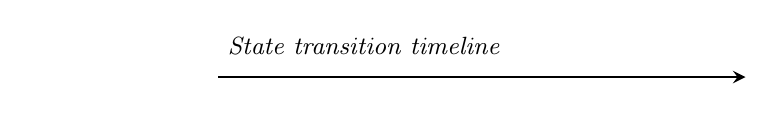
\begin{tikzpicture}
        \node at (0, 0) {};
        \node[anchor=west] at (2.3, 0.4) {{\small\it State transition timeline}};
        \draw [>=stealth,->,line width=1pt] (2.3, 0) to (9, 0);
    \end{tikzpicture}}\\
    \begin{tabular}{c|ccccccccccc}
      \hline
      $C_1$ & & \rdcircf{1} & & & & & & \rdcircf{7} & \blcircf{8} & & \\
      \hline
      $P$ & & & & \rdcircf{3} & & \rdcircf{5} & \blcircf{6} & & & \blcircf{9} & \\
      \hline
      $C_2$ & & & \blcircf{2} & & \rdcircf{4} & & & & & & \blcircf{10} \\
      \hline
    \end{tabular}\\
    \vspace{-10pt}\\
    $\downarrow$ (merge $[\rdcircf{3}; \rdcircf{4}; \rdcircf{5}]$ and $[\rdcircf{7}]$ by commuting $\blcircf{6}$ and $\rdcircf{7}$)\\
    \vspace{-10pt}\\
    \begin{tabular}{c|ccccccccccc}
      \hline
      $C_1$ & & \rdcircf{1} & & & & & \rdcircf{7} & & \blcircf{8} & & \\
      \hline
      $P$ & & & & \rdcircf{3} & & \rdcircf{5} & & \blcircf{6} & & \blcircf{9} & \\
      \hline
      $C_2$ & & & \blcircf{2} & & \rdcircf{4} & & & & & & \blcircf{10} \\
      \hline
    \end{tabular}\\
    \vspace{-10pt}\\
    $\downarrow$ (merge $[\rdcircf{1}]$ and $[\rdcircf{3}; \rdcircf{4}; \rdcircf{5}; \rdcircf{7}]$ by commuting $[\blcircf{2}]$ and $[\rdcircf{3}; \rdcircf{4}; \rdcircf{5}; \rdcircf{7}]$)\\
    \vspace{-10pt}\\
    \begin{tabular}{c|ccccccccccc}
      \hline
      $C_1$ & & \rdcircf{1} & & & & \rdcircf{7} & & & \blcircf{8} & & \\
      \hline
      $P$ & & & \rdcircf{3} & & \rdcircf{5} & & & \blcircf{6} & & \blcircf{9} & \\
      \hline
      $C_2$ & & & & \rdcircf{4} & & & \blcircf{2} & & & & \blcircf{10} \\
      \hline
    \end{tabular}
  \end{tabular}
  \caption{Serialization of an interleaved history by reductions}
  \label{fig-ex-sz-state-trs}
\end{figure}

\autoref{fig-ex-sz-state-trs} shows the original legal interleaved history (top) and how reductions apply to it and make it sequential (bottom).
In order to merge $[\rdcircf{3}; \rdcircf{4}; \rdcircf{5}]$ and $[\rdcircf{7}]$, either the commutation $\commhst{[\rdcircf{3}; \rdcircf{4}; \rdcircf{5}]}{[\blcircf{6}]}$ or $\commhst{[\blcircf{6}]}{[\rdcircf{7}]}$ should hold.
We will say that $[\blcircf{6}]$ is \emph{pushed} to the left (or right) when it commutes with $[\rdcircf{3}; \rdcircf{4}; \rdcircf{5}]$ (or $[\rdcircf{7}]$), respectively.

Two state transitions trivially commute if 1) the object state transitions happen in different objects and 2) input/output channels used for the transitions are all orthogonal to each other.
(We will formalize this intuition as a lemma in the actual serializability proof, shown in \autoref{sec-sz-proof}.)
If either of the conditions does not hold, we may need to analyze more.

\begin{figure}[t]
  \centering
  \begin{subfigure}[b]{0.48\textwidth}
    \begin{tikzpicture}
      % Alignment
      \node at (-3.6, 0) {};
      \node [anchor=north west,text width=2.5cm,inner sep=4pt,draw] at (-3.3, 0.4) {{\small \blmsgsm{rqI} and \rdmsgsm{rsM} are different, due to their message types.}};

      \node at (0, 0.5) {$P$};
      \node at (0, 0.15) {\tiny $5$};
      \draw [line width=0.2mm, >->] (0, 0) -- (0, -1.2);
      \node[label={[label distance=-4pt,myblue]right:{\small {\sf rqI}}},color=myblue] at (0, -0.4) {$\bullet$};
      \node[label={[label distance=-4pt,myred]right:{\small {\sf rsM}}},color=myred] at (0, -0.8) {$\bullet$};
      \node at (0, -1.5) {$C_1$};
      % Curves
      \draw [->,color=myblue] (1.1, 0.8) to[out=-135,in=90] node[below right] {\blcircflsm{6}{rqud}} (0.4, -0.1);
      \draw [->,color=myred] (0.4, -1.1) to[out=-90,in=90] node[right] {\rdcircflsm{7}{rsdd}} (0.4, -1.7);
    \end{tikzpicture}\medskip
    \caption{Reduction by different message types}
    \label{fig-ex-sz-comm-1}
  \end{subfigure}
  \begin{subfigure}[b]{0.48\textwidth}
    \begin{tikzpicture}
      % Alignment
      \node at (-3.5, 0) {};
      \node [anchor=north west,text width=0.9cm,inner sep=4pt,draw] at (-2.5, -0.3) {{\small silent}};
      \node [anchor=north west,text width=2.3cm,inner sep=4pt,draw] at (1.2, 0.4) {{\small \blmsgsm{rqM} and \rdmsgsm{rsI} use different channels.}};

      \node at (0, 0.5) {$P$};
      \node at (-0.2, 0.15) {\tiny $6$};
      \node at (0, 0.15) {\tiny $7$};
      \node at (0.2, 0.15) {\tiny $8$};
      \draw [line width=0.2mm, <-<] (-0.2, 0) -- (-0.2, -1.2);
      \draw [line width=0.2mm, <-<] (0, 0) -- (0, -1.2);
      \draw [line width=0.2mm, >->] (0.2, 0) -- (0.2, -1.2);
      \node[label={[label distance=-4pt,myblue]left:{\small {\sf rqM}}},color=myblue] at (-0.2, -0.4) {$\bullet$};
      \node[label={[label distance=-2pt,myred]left:{\small {\sf rsI}}},color=myred] at (0, -0.8) {$\bullet$};
      \node[label={[label distance=-4pt,myred]right:{\small {\sf rqI}}},color=myred] at (0.2, -0.8) {$\bullet$};
      \node at (0, -1.5) {$C_2$};
      % Curves
      \draw [->,color=myblue] (-0.7, -1.9) to[out=110,in=-90] node[left] {\blcircflsm{2}{rquu}} (-0.9, -0.7);
      \draw [->,color=myred] (0.6, -1.1) to[out=-90,in=-90,distance=1.4cm] node[right=5pt] {\rdcircflsm{4}{immu}} (-0.6, -1.1);
    \end{tikzpicture}
    \caption{Reduction by the rule-template properties}
    \label{fig-ex-sz-comm-2}
  \end{subfigure}
  \caption{Nontrivial reduction cases}
  \label{fig-ex-sz-comm}
\end{figure}

In the first merge case, $[\blcircf{6}]$ can be pushed to the right, \ie{} $(\commstep{\blcircf{6}}{\rdcircf{7}})$ holds.
The object state transitions are straightforward to deal with, since they are orthogonal ($P$ for $\blcircf{6}$ and $C_1$ for $\rdcircf{7}$).
It is nontrivial to deal with the used channels, however, since the output of $\blcircf{6}$ (\blmsgsm{rqI}) and the input of $\rdcircf{7}$ (\rdmsgsm{rsM}) share the same channel $5$.
\autoref{fig-ex-sz-comm-1} depicts this case; we see $\blcircf{6}$ and $\rdcircf{7}$ still commute, since \rdcircfl{7}{rsdd} should take a ``response'' (\rdmsgsm{rsM}) while \blcircfl{6}{rqud} outputs a ``request'' (\blmsgsm{rqI}).
It indicates that $\blcircf{6}$ and $\rdcircf{7}$ are involved with different messages in the same channel, thus not affecting commutativity.
After the merge, we obtain a new (less-interleaved) history, shown in the middle of \autoref{fig-ex-sz-state-trs}.

Now we should merge $[\rdcircf{1}]$ and $[\rdcircf{3}; \rdcircf{4}; \rdcircf{5}; \rdcircf{7}]$; in this case, $\blcircf{2}$ can be pushed to the right.
While this reduction is trivial in the sense of orthogonal objects and channels, the only nontrivial case is between $\blcircf{2}$ and $\rdcircf{4}$, where both rules are executed in $C_2$.
These state transitions still commute, as shown in \autoref{fig-ex-sz-comm-2}, since $\blcircf{2}$ cannot make any object state transition, according to the definition of the ``rquu'' rule template.
After this merge we finally obtain the sequential history.

How can we argue that the atomic-history fragments are always mergeable?
As we start to see in the two cases in \autoref{fig-ex-sz-state-trs}, mergeability \emph{follows from the rule templates}.
While trying to merge two fragments, we especially look at the rule template used in the last state transition of the first fragment and figure out which state transitions can be performed between the two.
For example, when checking mergeability between $[\rdcircf{3}; \rdcircf{4}; \rdcircf{5}]$ and $[\rdcircf{7}]$, we find that $\rdcircf{5}$ generates the output message \rdmsgsm{rsM}, and it blocks all the other transactions to go from $P$ to $C_1$, \eg{} $\blcircf{6}$ was blocked until $\rdcircf{7}$ consumes \rdmsgsm{rsM}.
We can thus commute $\blcircf{6}$ and $\rdcircf{7}$ due to this blocking.
In this sense, in proving serializability, we look at each rule template and characterize the allowed state transitions between two atomic-history fragments.

\section{The Formal Proof of Serializability}
\label{sec-sz-proof}

Based on the intuitions from \autoref{sec-sz-pf-intuition}, in this section we provide the formal proof of serializability.
The biggest contribution of the \hemiola{} framework includes precise formalization of the intuitions -- merging atomic fragments, commutativity among rule templates, left/right pushes, etc. -- and the serializability proof employing those intuitions.
The highest-level theorem will simply claim that use of good topology and the rule templates automatically guarantees serializability.

We will use the example of interleaving transactions shown in \autoref{fig-ex-sz-trs} throughout the proof for better understanding of the entire proof, referred to as the ``interleaving example.''

\subsection{Semi-sequential histories}
\label{sec-semi-seq-hst}

In \autoref{sec-sz-pf-intuition} we briefly provided the intuition of making a history sequential by merging atomic-history fragments repeatedly.
In order to employ the intuition in the actual proof, we need to show that \emph{finitely many} reductions suffice.
For example, while merging two atomic-history fragments, if we happen to separate the other fragment between the two, we will never be sure whether the merging process will be finished with the sequential history or not.

\begin{figure}[t]
  \centering
  \begin{tabular}{|c|}
    \hline
    \begin{math}
      \begin{array}{cc}
        \inference[STSilent:]{}{\strsn{S}{\listsingle{\lblEmpty{}}}} &
        \inference[STIns:]{}{\strsn{S}{\listsingle{\lblIns{\listof{m}}}}} \\[20pt]
        \inference[STOuts:]{}{\strsn{S}{\listsingle{\lblOuts{\listof{m}}}}} &
        \inference[STAtomic:]{\atomic{\listof{\amsgi{m}}}{\listof{l}}{\listof{\amsge{m}}}}{\strsn{S}{\listof{l}}} \\[20pt]
      \end{array}
    \end{math}\\
    \hline
  \end{tabular}
  \caption{Semi-transactions}
  \label{fig-semi-trs}
\end{figure}

What would be the way to say \emph{how much} a given history is sequentialized?
Semi-transactions are defined in order to have a quantitative progress measure for reductions.
The definition, given in \autoref{fig-semi-trs}, is almost the same as for (ordinary) transactions, except that an atomic history does not need to be external.
Thanks to this relaxation, any atomic-history fragment is a semi-transaction.

Semi-sequential histories are also defined in a similar way:
\begin{definition}[Semi-Sequential Histories]
  A history $h$ is \emph{semi-sequential} with \emph{degree} $n$ iff the history is a concatenation of $n$ semi-transactions.
  \begin{displaymath}
    \hsseq{S}{h}{n} \triangleq \exists\, \listof{t}.\; \sizeof{\listof{t}} = n \wedge (\forall t \in \listof{t}.\; \strsn{S}{t}) \wedge h = \listconcat{\listof{t}}.
  \end{displaymath}
\end{definition}
The only difference from sequential histories is that we \emph{count} the number of semi-transactions.
In our interleaving example, looking at the original interleaved history shown in \autoref{fig-ex-sz-state-trs}, we can find the following semi-transactions in-order: $[\rdcircf{1}]$, $[\blcircf{2}]$, $[\rdcircf{3}; \rdcircf{4}; \rdcircf{5}]$, $[\blcircf{6}]$, $[\rdcircf{7}]$, and $[\blcircf{8}; \blcircf{9}; \blcircf{10}]$.
In this case, the degree of a semi-sequential history is $6$, the number of semi-transactions.
Note that the degree of a semi-sequential history is not uniquely determined.
In the example, when regarding $[\rdcircf{3}; \rdcircf{4}; \rdcircf{5}]$ to the three separate single-label atomic histories -- $[\rdcircf{3}]$, $[\rdcircf{4}]$, and $[\rdcircf{5}]$ -- then we obtain another semi-sequential history with degree $8$.

This definition indicates that in order to obtain a serialized history, we should perform reductions to \emph{decrease the count as much as possible}.
\hemiola{} employs theorems that reflects this intuition:
\begin{theorem}
  \label{thm-sseq-default}
  Given a system $S$, a legal history is always semi-sequential:
  \begin{displaymath}
    \forall h.\; \semleg{S}{h} \to \exists n.\; \hsseq{S}{h}{n}.
  \end{displaymath}
\end{theorem}
\begin{proof}
  The proof is straightforward, since by definition any single-label history is a semi-transaction, and thus any history is semi-sequential, \ie{} $\forall h.\; \hsseq{S}{h}{\sizeof{h}}$.
\end{proof}

\begin{theorem}[Semi-sequentiality and serializability]
  \label{thm-sseq-sz}
  If $S$ satisfies the following property, then $S$ is serializable:
  \begin{align*}
    \forall h, n, s.\; & \semsteps{S}{\sysInit{S}}{h}{s} \land \hsseq{S}{h}{n} \to \\
    & \hseq{S}{h}\; \vee\\
    & \exists h_r, m.\; \semsteps{S}{\sysInit{S}}{h_r}{s} \wedge \hsseq{S}{h_r}{m} \wedge m < n.
  \end{align*}
\end{theorem}
\begin{proof}
  The proof employs the well-foundness of the less-than operator ($<$) for natural numbers.
  For a given history $h$ in a system $S$, we can find an initial number $n$ that satisfies $\hsseq{S}{h}{n}$ (by \autoref{thm-sseq-default}).
  Now by the given property, $h$ is either already sequential or reduces to $h_r$ with the degree $m < n$.
  Therefore, finite iteration of the property will eventually reduce the history to a sequential history.
\end{proof}

\subsection{Reduction of external input/output labels}
\label{sec-red-ext-labels}

For a given legal history in a system, the very first step to reduce it to a sequential history is to push all external input and output labels to the leftmost and rightmost regions of the history, respectively.
Recall that the serializability (\autoref{def-seq-sz}) does not require the sequential history to preserve the behavior of a history, but to reach to the same state.

The following two dual theorems are enough to push all external labels:
\begin{theorem}
  \label{thm-push-ext-labels}
  In any legal history in the system $S$, the first external-input (or the last external-output) label can be pushed to the first (or the last) of the history, respectively:
  \begin{displaymath}
    \forall s_0, s_1, \listof{h_0}, im, \listof{h_1}.\;
    \mathsf{NoExtIns}(\listof{h_0}) \to
    \semsteps{S}{s_0}{\listapp{\listcons{\listof{h_0}}{\lblIns{im}}}{\listof{h_1}}}{s_1} \to
    \semsteps{S}{s_0}{\listapp{\lblIns{im}}{\listapp{\listof{h_0}}{\listof{h_1}}}}{s_1}\ \textrm{and}
  \end{displaymath}
  \begin{displaymath}
    \forall s_0, s_1, \listof{h_0}, im, \listof{h_1}.\;
    \mathsf{NoExtOuts}(\listof{h_1}) \to
    \semsteps{S}{s_0}{\listapp{\listcons{\listof{h_0}}{\lblOuts{im}}}{\listof{h_1}}}{s_1} \to
    \semsteps{S}{s_0}{\listapp{\listapp{\listof{h_0}}{\listof{h_1}}}{\lblOuts{im}}}{s_1},
  \end{displaymath}
  where $\mathsf{NoExtIns}(\listof{h}) \triangleq \forall l.\; l \in \listof{h} \to \forall im.\; l \neq \lblIns{im}$ and
  $\mathsf{NoExtOuts}(\listof{h}) \triangleq \forall l.\; l \in \listof{h} \to \forall im.\; l \neq \lblOuts{im}$.
\end{theorem}
\begin{proof}
  By definition it suffices to prove \commhst{\listof{h_0}}{\listsingle{\lblIns{im}}}.
  Since $\mathsf{NoExtIns}(\listof{h_0})$, each label in $\listof{h_0}$ is a silent, external-output, or internal label.
  It is trivial that a silent label and an external-input label commute, since the silent label makes no state transition.
  An external-output label and an external-input label also commute, since they use different channels.
  Commutativity between an internal label and an external-input label is relatively nontrivial, since an internal label may dequeue some external inputs.
  They still commute, however, since dequeue of an external-input label means there is already an external input message in the channel, and the external-input label adds a different message to the system.
  The proof for the external-output label is almost same as the one for the external-input label.
\end{proof}

\tikzset{
  ->-/.style={
    decoration={
      markings,
      mark=at position #1 with {\arrow{>}}},
    postaction={decorate}
  }
}
\begin{figure}[h]
  \centering
  \begin{tikzpicture}
    \draw[->-=0.5] (-0.8, 0) -- (-0.4, 0);
    \draw[fill=myred, text=white] (0,0) circle [radius=0.4] node {$l^0_{\textrm{in}}$};
    \draw[->-=0.5] (0.4, 0) -- (0.8, 0);
    \draw[fill=mygray, text=white] (1.2,0) circle [radius=0.4] node {$l^0_{\textrm{int}}$};
    \draw[->-=0.5] (1.6, 0) -- (2.0, 0);
    \draw[fill=myblue, text=white] (2.4,0) circle [radius=0.4] node {$l^0_{\textrm{out}}$};
    \draw[->-=0.5] (2.8, 0) -- (3.2, 0);
    \draw[fill=myred, text=white] (3.6,0) circle [radius=0.4] node {$l^1_{\textrm{in}}$};
    \draw[->-=0.5] (4.0, 0) -- (4.4, 0);
    \draw[fill=mygray, text=white] (4.8,0) circle [radius=0.4] node {$l^1_{\textrm{int}}$};
    \draw[->-=0.5] (5.2, 0) -- (5.6, 0);
    \draw[fill=myblue, text=white] (6,0) circle [radius=0.4] node {$l^1_{\textrm{out}}$};
    \draw[->-=0.5] (6.4, 0) -- (6.8, 0);

    \node at (3.0, -1.0) {\small $\downarrow^{\ast}$ (after some reductions)};

    \draw[->-=0.5] (-0.8, -2.0) -- (-0.4, -2.0);
    \draw[fill=myred, text=white] (0,-2.0) circle [radius=0.4] node {$l^0_{\textrm{in}}$};
    \draw[->-=0.5] (0.4, -2.0) -- (0.8, -2.0);
    \draw[fill=myred, text=white] (1.2,-2.0) circle [radius=0.4] node {$l^1_{\textrm{in}}$};
    \draw[->-=0.5] (1.6, -2.0) -- (2.0, -2.0);
    \draw[fill=mygray, text=white] (2.4,-2.0) circle [radius=0.4] node {$l^0_{\textrm{int}}$};
    \draw[->-=0.5] (2.8, -2.0) -- (3.2, -2.0);
    \draw[fill=mygray, text=white] (3.6,-2.0) circle [radius=0.4] node {$l^1_{\textrm{int}}$};
    \draw[->-=0.5] (4.0, -2.0) -- (4.4, -2.0);
    \draw[fill=myblue, text=white] (4.8,-2.0) circle [radius=0.4] node {$l^0_{\textrm{out}}$};
    \draw[->-=0.5] (5.2, -2.0) -- (5.6, -2.0);
    \draw[fill=myblue, text=white] (6,-2.0) circle [radius=0.4] node {$l^1_{\textrm{out}}$};
    \draw[->-=0.5] (6.4, -2.0) -- (6.8, -2.0);
  \end{tikzpicture}
  \caption{Pushing all external input/output labels}
  \label{fig-reducing-exts}
\end{figure}

\autoref{fig-reducing-exts} shows an original example history and the resulting history after pushing all the external input and output labels in the original history.
We can generate such a history by performing reductions:
\begin{itemize}
\item Try to pick the first external-input label that is \emph{not in the leftmost region of the history yet}. If it exists, it can always be pushed to the left, right after the external-input labels that are already in the leftmost region, by applying \autoref{thm-push-ext-labels}.
\item Try to pick the last external output label that is \emph{not at the rightmost region of the history yet}. If it exists, it can always be pushed to the right, right before the external-output labels that are already in the rightmost region, by applying \autoref{thm-push-ext-labels}.
\end{itemize}
Note that pushing the external input (output) labels to the leftmost (rightmost), respectively, is possible since the semantics of the protocol transition system is based on infinite-sized buffers, allowing the system to accept all the external input messages as early as possible and to postpone releasing all the external output messages as late as possible.

\subsection{Interleaving and nonconfluent histories}
\label{sec-itlv-ncf-hst}

Now we formalize the atomic-history fragments mentioned in \autoref{sec-sz-pf-intuition} -- whether the two fragments belong to the same transaction or not.
From this section, we will just deal with histories only consisting of internal labels, to focus on how to serialize atomic histories, assuming external labels are already pushed to the edges by the method described in \autoref{sec-red-ext-labels}.

The below notion of continuity lets us figure out whether two histories are related as adjacent parts of a whole atomic history:
\begin{definition}[Continuity]\mbox{}\vspace{-8pt}\\
  \begin{enumerate}
  \item Two atomic histories $h_1$ and $h_2$ are continuous (\hcontsymb{}) iff the initial messages of $h_2$ are in the live messages of $h_1$:
    \begin{displaymath}
      \hcont{h_1}{h_2}\; \triangleq\quad \atomic{\listof{\amsgi{im_1}}}{h_1}{\listof{\amsge{im_1}}} \;\wedge\; \atomic{\listof{\amsgi{im_2}}}{h_2}{\listof{\amsge{im_2}}} \;\wedge\; \listof{\amsgi{im_2}} \subseteq \listof{\amsge{im_1}}.
    \end{displaymath}
  \item We say $h_1$ and $h_2$ are externally continuous (denoted as $\hextcont{S}{h_1}{h_2}$) if they are continuous and $h_1$ is externally atomic.
  \item Two atomic histories $h_1$ and $h_2$ are discontinuous iff the live messages of $h_1$ are disjoint from the initial messages of $h_2$:
    \begin{displaymath}
      \hdiscont{h_1}{h_2}\; \triangleq\quad \atomic{\listof{\amsgi{im_1}}}{h_1}{\listof{\amsge{im_1}}} \;\wedge\; \atomic{\listof{\amsgi{im_2}}}{h_2}{\listof{\amsge{im_2}}} \;\wedge\; \listdisj{\listof{\amsge{im_1}}}{\listof{\amsgi{im_2}}}.
    \end{displaymath}
  \end{enumerate}
\end{definition}
Note that the discontinuity requires that the live messages of the previous history are \emph{disjoint} to the initial messages of the next history.
Therefore, it is not true that two atomic histories are always either continuous or discontinuous.
We will very soon explore how to deal with the other case, where the next history takes multiple sets of live messages from the previous histories.

From now on, throughout this chapter, we will have a number of definitions that use a sequence of atomic histories.
Such a sequence $\listof{h}$ will be predicated as $\atomicHsts{\listof{h}}$, with the following formal definition:
$\atomicHsts{\listof{h}} \triangleq \forall h \in \listof{h}.\; \atomicShort{h}$.

Using the notion of continuity, we can also formalize interleaving of atomic histories:
\begin{definition}[Interleaved Histories]
  In a given system $S$, a sequence of atomic histories $\listof{h}$ is interleaved iff there exist two histories $h_1$ and $h_2$ in the sequence that are externally continuous and any history between the two is discontinuous to $h_1$:
  \begin{align*}
    \hitlv{S}{\listof{h}}\; \triangleq\quad & \atomicHsts{\listof{h}}\; \wedge\\
    & \exists h_1, h_2, \listof{h_1}, \listof{h_2}, \listof{h_3}. \\
    & \listof{h} = \listapp{\listcons{\listapp{\listcons{\listof{h_1}}{h_1}}{\listof{h_2}}}{h_2}}{\listof{h_3}}\; \wedge \\
    & \hextcont{S}{h_1}{h_2} \wedge (\forall h' \in \listof{h_2}.\; \hdiscont{h_1}{h'}).
  \end{align*}
  We also call a history $h$ interleaved, overrided as $(\hitlv{S}{h})$, iff we can find an interleaved sequence of histories $\listof{h_s}$ that satisfies $h = \listconcat{\listof{h_s}}$.
\end{definition}

There are two subtleties in defining the notion of interleaving precisely.
First, we look for \emph{externally continuous} histories, not just continuous ones, to define whether the whole history is interleaved or not.
It does not restrict the notion since when continuous histories are found in a legal history, either they are already externally continuous or the ones are found at the beginning of the atomic-history chain that contains them.
Second, we require that the earlier history ($h_1$) is \emph{discontinuous} to each history ($\forall h' \in \listof{h_2}$) between the two externally continuous histories ($h_1$ and $h_2$).
This is to ensure that the live messages generated by $h_1$ are preserved -- \ie{} not consumed by some other atomic histories -- until $h_2$ takes its initial messages from those ones.

Note that our interleaving example is indeed interleaved: we can find externally continuous histories $[\rdcircf{1}]$ and $[\rdcircf{3}; \rdcircf{4}; \rdcircf{5}]$, and $[\rdcircf{1}]$ is discontinuous with the only intermediate atomic history $[\blcircf{2}]$.

One of the main intuitions to prove serializability is to categorize a given history.
If the history is already sequential, we do not need to proceed further.
If the history is interleaved, we will need to merge the externally continuous histories, which will decrease the degree of semi-sequentiality and lead to a sequential history.
This categorization, however, implicitly assumes any history is either sequential or interleaved.

\begin{figure}
  \centering
  \begin{tabular}{cc}
    \begin{tabular}{c}
      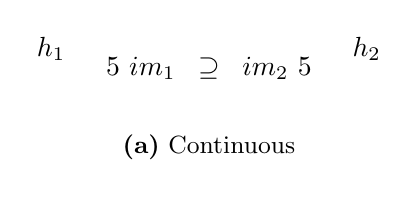
\begin{tikzpicture}
        \node[anchor=east] at (-1.4, 0.25) {$h_1$};
        \node[anchor=east] at (0.0, 0) {$\squigs{5}\rsquigend\ \listof{\amsge{im_1}}$};
        \node at (0.3, 0) {$\supseteq$};
        \node[anchor=west] at (2.0, 0.25) {$h_2$};
        \node[anchor=west] at (0.6, 0) {$\listof{\amsgi{im_2}}\ \squigs{5}\rsquigend$};
        \node at (0.3, -1.0) {{\small{\bf (a)} Continuous}};
      \end{tikzpicture} \\
      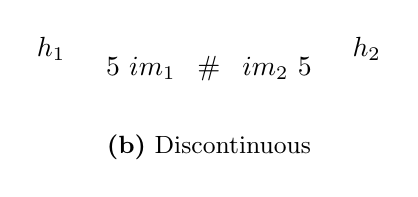
\begin{tikzpicture}
        \node[anchor=east] at (-1.4, 0.25) {$h_1$};
        \node[anchor=east] at (0.0, 0) {$\squigs{5}\rsquigend\ \listof{\amsge{im_1}}$};
        \node at (0.3, 0) {$\#$};
        \node[anchor=west] at (2.0, 0.25) {$h_2$};
        \node[anchor=west] at (0.6, 0) {$\listof{\amsgi{im_2}}\ \squigs{5}\rsquigend$};
        \node at (0.3, -1.0) {{\small{\bf (b)} Discontinuous}};
      \end{tikzpicture}
    \end{tabular} &
    \adjustbox{valign=c}{
      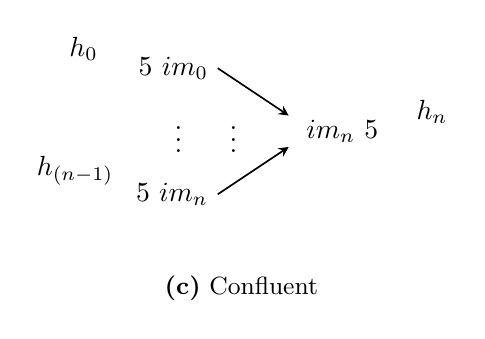
\begin{tikzpicture}
        \node[anchor=east] at (-1.4, 1.05) {$h_0$};
        \node[anchor=east] at (0.0, 0.8) {$\squigs{5}\rsquigend\ \listof{\amsge{im_0}}$};
        \node at (-0.5, 0) {$\vdots$};
        \node[anchor=east] at (-1.2, -0.5) {$h_{(n-1)}$};
        \node[anchor=east] at (0.0, -0.8) {$\squigs{5}\rsquigend\ \listof{\amsge{im_n}}$};

        \node[anchor=west] at (2.4, 0.25) {$h_n$};
        \node[anchor=west] at (1.0, 0) {$\listof{\amsgi{im_n}}\ \squigs{5}\rsquigend$};

        \draw [->, >=stealth, line width=0.6pt] (0.0, 0.8) -- (0.9, 0.2);
        \node at (0.2, 0) {$\vdots$};
        \draw [->, >=stealth, line width=0.6pt] (0.0, -0.8) -- (0.9, -0.2);

        \node at (0.3, -2.0) {{\small{\bf (c)} Confluent}};
      \end{tikzpicture}}\\
  \end{tabular}
  \caption{Three relation types between atomic histories}
  \label{fig-atomic-hst-three-types}
\end{figure}

An additional condition is required, unfortunately, just to reason with sequential and interleaved histories.
In other words, there is a third type of a history, happening when at least two different external atomic histories come together via a local state transition consuming some live messages of these histories.
\autoref{fig-atomic-hst-three-types} depicts the three types of relations between two atomic histories.
While atomic-history fragments in an interleaved history are only expected to be continuous or discontinuous to each other, there is another relation type, which is called \emph{confluent} histories.
This confluence case does not happen in any practical cache-coherence protocols, but we still need a formal predicate to ensure that the target system never generates such cases.

The \emph{nonconfluence} predicate removes this case, by claiming that any atomic history is either the start of a new transaction or a continuation of a previous transaction:
\newcommand{\sncf}[1]{\ensuremath{\mathsf{Nonconfluent}\ #1}}
\begin{definition}[Nonconfluence]
  \label{def-ncf}
  A system $S$ is \emph{nonconfluent} iff any first non-external history (if it exists) is interleaved (with an external atomic history):
  \begin{displaymath}
    \begin{array}{rcl}
      \sncf{S}\; \triangleq\quad & \forall \listof{h}, h_0, s. &
      \atomicHsts{\listcons{\listof{h}}{h_0}} \;\wedge\\
      & & \semsteps{S}{\sysInit{S}}{\listapp{\listconcat{\listof{h}}}{h_0}}{s}
      \wedge\; (\forall h \in \listof{h}.\; \extatomicShort{S}{h})
      \wedge\; \neg(\extatomicShort{S}{h_0}) \to\\
      & & \hitlv{S}{(\listcons{\listof{h}}{h_0})}.
    \end{array}
  \end{displaymath}
\end{definition}

\subsection{Merging interleaved histories}

In the last section, we examined the three types of histories and showed that the nonconfluence property rules out all confluent histories, so it is safe to reason only with interleaved histories.
(Sequential histories are already good in terms of serializability.)
In \autoref{sec-sz-pf-intuition} we provided our intuition that an interleaved history will be reduced to a sequential history by repeatedly merging atomic-history fragments.
In this section, we provide the formal definition of such merges and show that the nonconfluence and mergeability properties imply serializability.

As mentioned in \autoref{sec-itlv-ncf-hst}, the main purpose of merging two continuous histories is to decrease the degree of semi-sequentiality, so we have a less-interleaved history.
Focusing solely on this purpose, we formally define the notion of mergeability as follows:
\begin{definition}[Mergeability]
  \label{def-mgb}
  For a given system $S$, two histories $h_1$ and $h_2$ are \emph{mergeable} iff any history containing the two histories can be reduced to the one where the two histories are merged and the number of atomic-history fragments for the other histories is preserved:
  \begin{displaymath}
    \begin{array}{rrl}
      \hmgb{S}{h_1}{h_2}\; \triangleq & \forall s_1. & \semrch{S}{s_1} \to\\
      & \forall \listof{h}, s_2. & \atomicHsts{\listof{h}} \;\wedge\;
      \semsteps{S}{s_1}{\listapp{h_1}{\listapp{\listconcat{\listof{h}}}{h_2}}}{s_2} \to\\
      & \exists \listof{h}_{\textrm{l}}, \listof{h}_{\textrm{r}}.
      & \atomicHsts{\listof{h}_{\textrm{l}}} \;\wedge\; \atomicHsts{\listof{h}_{\textrm{r}}} \;\wedge\\
      & & \semsteps{S}{s_1}{\listapp{\listconcat{\listof{h_{\textrm{l}}}}}{\listapp{h_1}{\listapp{h_2}{\listconcat{\listof{h_{\textrm{r}}}}}}}}{s_2} \;\wedge\; \sizeof{\listof{h}} = \sizeof{\listof{h_{\textrm{l}}}} + \sizeof{\listof{h_{\textrm{r}}}}.
    \end{array}
  \end{displaymath}
  Furthermore, we say the system $S$ is \emph{mergeable} if any externally continuous histories in a legal history are mergeable:
  \begin{displaymath}
    \smgb{S} \triangleq \forall h_1, h_2.\; \hextcont{S}{h_1}{h_2} \to \hmgb{S}{h_1}{h_2}.
  \end{displaymath}
\end{definition}

The mergeability definition is abstract in that it relates the intermediate histories ($\listof{h}$) and the pushed histories ($\listof{h_{\textrm{l}}}$ and $\listof{h_{\textrm{r}}}$) not by mentioning they are indeed pushed from $\listof{h}$, but just by requiring \emph{the number of atomic-history fragments are preserved} ($\sizeof{\listof{h}} = \sizeof{\listof{h_{\textrm{l}}}} + \sizeof{\listof{h_{\textrm{r}}}}$).
This condition implies that the number of atomic-history fragments is preserved after the merge.
When $h_1$ and $h_2$ are continuous histories, however, by merging $h_1$ and $h_2$ we get the entire number of fragments decreased by 1, which means that the history after the merge has a smaller semi-sequentiality degree.

We are finally equipped with enough definitions to introduce a convenient general way to prove serializability:
\begin{theorem}
  If a system $S$ is nonconfluent and mergeable, then it is serializable.
  \begin{displaymath}
    \forall S.\; \sncf{S} \land \smgb{S} \to \hsrz{S}.
  \end{displaymath}
  \vspace{-15pt}
  \label{thm-sz-when}
\end{theorem}
\begin{proof}
  For a given history $h$, by \autoref{thm-sseq-sz} there exists a sequence of atomic histories $\listof{h_s}$ such that $\listconcat{\listof{h_s}} = h$.
  In the sequence we try to find the first externally continuous histories.
  If we cannot find the ones, then by definition $h$ is already sequential.
  If there exist such histories, by the definition of nonconfluence (\autoref{def-ncf}) they are interleaved.
  Now by mergeability (\autoref{def-mgb}) we can find a new sequence of histories $\listof{h_r}$ that reaches the same state, where the externally continuous histories are merged, thus $\sizeof{\listof{h_r}} < \sizeof{\listof{h}}$.
  Applying \autoref{thm-sseq-sz}, we will eventually obtain a sequential history reaching the same state by repeating this process.
\end{proof}

\subsection{Reduction and pushes by separation}

\newcommand{\aobjs}[1]{\ensuremath{\mathsf{objs}\,(#1)}}
\newcommand{\achns}[1]{\ensuremath{\mathsf{chns}\,(#1)}}
\newcommand{\ainputs}[1]{\ensuremath{\mathsf{ins}\,(#1)}}
\newcommand{\aoutputs}[1]{\ensuremath{\mathsf{outs}\,(#1)}}
\newcommand{\ainits}[1]{\ensuremath{\mathsf{inits}\,(#1)}}
\newcommand{\alives}[1]{\ensuremath{\mathsf{lives}\,(#1)}}
\newcommand{\objsep}[2]{\ensuremath{\mathsf{ObjSep}\ #1\ #2}}
\newcommand{\objseph}[2]{\ensuremath{\mathsf{ObjSepHst}\ #1\ #2}}
\newcommand{\msgseph}[2]{\ensuremath{\mathsf{MsgSepHst}\ #1\ #2}}
\newcommand{\stseph}[2]{\ensuremath{\mathsf{SepHst}\ #1\ #2}}

\autoref{thm-sz-when} presents a good intuition on how to prove serializability using nonconfluence and mergeability.
The mergeability definition (\autoref{def-mgb}), however, is rather abstract; it does not provide any actual techniques to merge continuous histories.
In this section, we explore a method to merge continuous histories, by using \emph{state-transition separation} and \emph{pushability}.

\subsubsection{Reduction by separation}

We begin with introducing the trivial reduction between two state transitions:
\begin{theorem}
  \label{thm-red-trivial-steps}
  Two state transitions commute if they affect different objects and different input/output channels:
  \begin{displaymath}
    \renewcommand{\arraystretch}{1.2}
    \begin{array}{l}
      \forall o_1, r_1, \listof{\mathrm{ins}}_1, \listof{\mathrm{outs}}_1,
      o_2, r_2, \listof{\mathrm{ins}}_2, \listof{\mathrm{outs}}_2.\\
      \quad\quad o_1 \neq o_2 \;\wedge\; \listdisj{(\listof{\idxOf{\mathrm{ins}_1}} \cup \listof{\idxOf{\mathrm{outs}_1}})}{(\listof{\idxOf{\mathrm{ins}_2}} \cup \listof{\idxOf{\mathrm{outs}_2}})} \to\\
      \quad\quad \commstep{\lblInt{o_1}{r_1}{\listof{\mathrm{ins}}_1}{\listof{\mathrm{outs}}_1}}
                 {\lblInt{o_2}{r_2}{\listof{\mathrm{ins}}_2}{\listof{\mathrm{outs}}_2}}.
    \end{array}
  \end{displaymath}
\end{theorem}

For a given history $h$, we denote by \aobjs{h} (\achns{h}) the set of object (channel) indices whose state is \emph{used} by $h$, obtained by collecting the object index (the input/output channel indices) in each label in $h$, respectively.
We can then lift the trivial reduction theorem to the one for histories, using \aobjs{h} and \achns{h}:
\begin{theorem}[Reduction by trivial separation]
  \label{thm-red-trivial-hsts}
  Two histories commute if they affect different objects and different input/output channels:
  \begin{displaymath}
    \forall h_1, h_2.\; \listdisj{\aobjs{h_1}}{\aobjs{h_2}} \;\wedge\; \listdisj{\achns{h_1}}{\achns{h_2}} \to \commhst{h_1}{h_2}.
  \end{displaymath}
\end{theorem}

\autoref{thm-red-trivial-hsts} is too trivial to be used in actual atomic histories generated by the \hemiola{} DSL.
We thus relax this theorem with respect to object and message states, so it can be used in the actual serializability proof.

Firstly, instead of comparing object indices, \aobjs{h_1} and \aobjs{h_2}, sometimes we would like to prove the commutativity of state transitions \emph{within an object} directly.
Given two internal labels \lblInt{\idxOf{O}}{\idxOf{r_1}}{\listof{\mathrm{ins}}_1}{\listof{\mathrm{outs}}_1} and \lblInt{\idxOf{O}}{\idxOf{r_2}}{\listof{\mathrm{ins}}_2}{\listof{\mathrm{outs}}_2} (created by the same object $O$), if we prove the following property then the two labels are commutative in terms of object state transitions:
\begin{displaymath}
  \renewcommand{\arraystretch}{1.2}
  \begin{array}{rl}
    \objsep{r_1}{r_2} \triangleq & \forall o_0, \listof{\mathrm{ins}}_1, \listof{\mathrm{ins}}_2.\\
    & \mathsf{let}\ (o_1, \listof{\mathrm{outs}}_1) := \rtrsOf{r_1}\;(o_0, \listof{\mathrm{ins}}_1)\ \mathsf{in}\\
    & \mathsf{let}\ (o_2, \listof{\mathrm{outs}}_2) := \rtrsOf{r_2}\;(o_1, \listof{\mathrm{ins}}_2)\ \mathsf{in}\\
    & \mathsf{let}\ (o_1', \listof{\mathrm{outs}}_2') := \rtrsOf{r_2}\;(o_0, \listof{\mathrm{ins}}_2)\ \mathsf{in}\\
    & \listof{\mathrm{outs}}_2 = \listof{\mathrm{outs}}_2' \;\wedge\;
    \rtrsOf{r_1}\;(o_1', \listof{\mathrm{ins}}_1) = (o_2, \listof{\mathrm{outs}}_1).
  \end{array}
\end{displaymath}
For instance, while using the \hemiola{} DSL, when an object forwards an upward request it sets an uplock.
The object should be able to handle a downward request to it even after setting the uplock.
These two state transitions are always commutative, since there is no state transition while forwarding the upward request (except locking) and handling the downward request does not affect the uplock.

This object separation is naturally extended to the one for atomic histories:
\begin{definition}\label{def-obj-comm}
  For given atomic histories $h_1$ and $h_2$, we say $h_1$ and $h_2$ are object-separated, denoted as $(\objseph{h_1}{h_2})$, if the following conditions are satisfied:
  \begin{displaymath}
    \renewcommand{\arraystretch}{1.2}
    \begin{array}{rcl}
      \objseph{h_1}{h_2} \triangleq & \forall l_1, l_2. & l_1 \in h_1 \;\wedge\; l_2 \in h_2 \to\\
      & & \mathsf{let}\ \lblInt{\idxOf{O_1}}{\idxOf{r_1}}{\listof{\mathrm{ins}}_1}{\listof{\mathrm{outs}}_1} := l_1\ \mathsf{in}\\
      & & \mathsf{let}\ \lblInt{\idxOf{O_2}}{\idxOf{r_2}}{\listof{\mathrm{ins}}_2}{\listof{\mathrm{outs}}_2} := l_2\ \mathsf{in}\\
      & & \idxOf{O_1} \neq \idxOf{O_2} \;\vee\; (\idxOf{O_1} = \idxOf{O_2} \;\wedge\; \objsep{r_1}{r_2}).
    \end{array}
  \end{displaymath}
\end{definition}
Note that each label $l$ in $h_1$ (or $h_2$) is always an internal label, since it is an atomic history.
The intuition here is that $h_1$ and $h_2$ are commutative in terms of object state transitions when each label -- representing an object state transition -- in $h_1$ and $h_2$ are commutative either by different objects (separation) or by the commutativity conditions within the same object.

Next we consider message states.
Instead of comparing channel indices regardless of their input/output types, we relax the notion to allow the live messages of $h_1$ and the initial messages of $h_2$ to be in the same channel but still different.
We first define a couple of new notions for atomic histories:
\begin{definition}
  For given an atomic history $h$, we define the input and output messages of $h$, denoted as \ainputs{h} and \aoutputs{h}, respectively:
  \begin{displaymath}
    \renewcommand{\arraystretch}{1.2}
    \begin{array}{l}
      \ainputs{h} \triangleq \listconcat{(\mathsf{List.map}\ (\lambda l.\; \mathsf{let}\ \lblInt{o}{r}{\listof{\mathrm{ins}}}{\listof{\mathrm{outs}}} := l\ \mathsf{in}\ \listof{\idxOf{\mathrm{ins}}})\ h)}.\\
      \aoutputs{h} \triangleq \listconcat{(\mathsf{List.map}\ (\lambda l.\; \mathsf{let}\ \lblInt{o}{r}{\listof{\mathrm{ins}}}{\listof{\mathrm{outs}}} := l\ \mathsf{in}\ \listof{\idxOf{\mathrm{outs}}})\ h)}.
    \end{array}
  \end{displaymath}
\end{definition}
As seen in the definition, \ainputs{h} (or \aoutputs{h}) collects all the input (output) message channels of the internal labels, respectively.
We will also use \ainits{h} and \alives{h} to refer to the initial messages and live messages of $h$, respectively.

\begin{definition}\label{def-msg-comm}
  For given atomic histories $h_1$ and $h_2$, we say $h_1$ and $h_2$ are message-separated, denoted as $(\msgseph{h_1}{h_2})$, if the following conditions are satisfied:
  \begin{displaymath}
    \renewcommand{\arraystretch}{1.2}
    \begin{array}{rl}
      \msgseph{h_1}{h_2} \triangleq & \forall\; \listof{\mathrm{inits}}_1, \listof{\mathrm{lives}}_1, \listof{\mathrm{inits}}_2, \listof{\mathrm{lives}}_2.\\
      & \atomic{\listof{\mathrm{inits}}_1}{h_1}{\listof{\mathrm{lives}}_1} \;\wedge\;
      \atomic{\listof{\mathrm{inits}}_2}{h_2}{\listof{\mathrm{lives}}_2} \to\\
      & \listdisj{\ainputs{h_1}}{\ainputs{h_2}} \;\wedge\;
      \listdisj{\ainputs{h_1}}{\aoutputs{h_2}} \;\wedge\\
      & \listdisj{\listof{\mathrm{lives}}_1}{\listof{\mathrm{inits}}_2} \;\wedge\;
      \listdisj{\aoutputs{h_1}}{\aoutputs{h_2}}.
    \end{array}
  \end{displaymath}
\end{definition}
Instead of having $\listdisj{\achns{h_1}}{\achns{h_2}}$ as a disjointness condition, we see a relaxation between $\listof{\mathrm{lives}}_1$ and $\listof{\mathrm{inits}}_2$ to require disjointness not only by channel indices, but also by message values.

This relaxation is indeed required to prove serializability in \hemiola{}.
We can find an instance from our interleaving example, again, specifically from \autoref{fig-ex-sz-comm-1}.
It is the case where the atomic history $[\blcircf{6}]$ happens first, generating \blmsgsm{rqI} to the channel $5$ as the live message, and the atomic history $[\rdcircf{7}]$ happens next, consuming \rdmsgsm{rsM} from the same channel.
These two histories commute, but if we just use \autoref{thm-red-trivial-hsts} with the trivial conditions, we cannot prove the commutativity.
We can employ the relaxed condition (\autoref{def-msg-comm}), though, since \blmsgsm{rqI} and \rdmsgsm{rsM} are different messages thus the relaxed condition $\listdisj{\listof{\mathrm{lives}}_1}{\listof{\mathrm{inits}}_2}$ holds.

Using the new, relaxed object and message separations, we present the following reduction theorem:
\begin{theorem}[Reduction by separation]
  \label{thm-red-by-sep}
  \begin{displaymath}
    \forall h_1, h_2.\; \atomicShort{h_1} \;\wedge\; \atomicShort{h_2} \;\wedge\; \stseph{h_1}{h_2} \to \commhst{h_1}{h_2},
  \end{displaymath}
  where $\stseph{h_1}{h_2} \triangleq \objseph{h_1}{h_2} \;\wedge\; \msgseph{h_1}{h_2}$.
\end{theorem}
\begin{proof}
  The proof is quite straightforward by nested induction on \atomicShort{h_1} and \atomicShort{h_2}.
  The base case is to prove \commstep{l_1}{l_2} when $h_1 = \listsingle{l_1}$ and $h_2 = \listsingle{l_2}$.
  Suppose $l_1 = \lblInt{\idxOf{O_1}}{\idxOf{r_1}}{\listof{\mathrm{ins}}_1}{\listof{\mathrm{outs}}_1}$ and $l_2 = \lblInt{\idxOf{O_2}}{\idxOf{r_2}}{\listof{\mathrm{ins}}_2}{\listof{\mathrm{outs}}_2}$.
  Then we obtain the object separation $(\objsep{r_1}{r_2})$ from $(\objseph{h_1}{h_2})$.
  We also obtain $\listdisj{\listof{\idxOf{\mathrm{ins}_1}}}{\listof{\idxOf{\mathrm{ins}_2}}}$,
  $\listdisj{\listof{\idxOf{\mathrm{ins}_1}}}{\listof{\idxOf{\mathrm{outs}_2}}}$,
  $\listdisj{\listof{\mathrm{outs}_1}}{\listof{\mathrm{ins}_2}}$, and
  $\listdisj{\listof{\idxOf{\mathrm{outs}_1}}}{\listof{\idxOf{\mathrm{outs}_2}}}$ from $(\msgseph{h_1}{h_2})$.
  These conditions are enough to prove commutativity between $l_1$ and $l_2$ just by construction.
  Induction cases are straightforward as well, \eg{} if $h_1 = \listcons{h_1'}{l_1}$ we perform reduction between $l_1$ and $h_2$ first, and do another reduction between $h_1'$ and $h_2$ by the induction hypothesis to perform the whole reduction between $h_1$ and $h_2$.
\end{proof}

\subsubsection{Pushes by separation}

Now we provide our method to merge continuous histories, by pushing all intermediate atomic-history fragments outside of the continuous histories.
Pushing an intermediate atomic-history fragment will require a finite number of history reductions, and we will use \autoref{thm-red-by-sep} for each one.

Suppose that we want to merge continuous histories $h_1$ and $h_2$ through the intermediate atomic histories $\listof{h}$.
We first categorize each atomic history into two groups: \emph{left-pushable} histories and \emph{right-pushable} histories, with the following requirements:
\begin{enumerate}
\item $h_1$ and a left-pushable history are always commutative:
  \begin{displaymath}
    \forall h \in \listof{h}.\; \mathsf{LeftPushable}\ h \to \commhst{h_1}{h}.
  \end{displaymath}
\item A right-pushable history and $h_2$ are always commutative:
  \begin{displaymath}
    \forall h \in \listof{h}.\; \mathsf{RightPushable}\ h \to \commhst{h}{h_2}.
  \end{displaymath}
\item A right-pushable history and a left-pushable one are always commutative:
  \begin{displaymath}
    \forall h_r, h_l \in \listof{h}.\; \mathsf{RightPushable}\ h_r \to \mathsf{LeftPushable}\ h_l \to \commhst{h_r}{h_l}.
  \end{displaymath}
\end{enumerate}

These three conditions are enough to merge $h_1$ and $h_2$.
\begin{theorem}\label{thm-push-imp-mgb}
  If each $h \in \listof{h}$ can be categorized in terms of left/right pushability, then \hmgb{S}{h_1}{h_2} holds.
\end{theorem}
\begin{proof}
  We first try to find the first left-pushable history in $\listof{h}$.
  If it does not exist, then all the atomic-history fragments in $\listof{h}$ are right-pushable.
  In this case $\commhst{\listconcat{\listof{h}}}{h_2}$ holds by repeatedly commuting the last fragment of \listof{h} and $h_2$.
  If it exists, suppose $\listof{h} = \listapp{\listcons{\listof{h_r}}{h_l}}{\listof{h_e}}$, where $h_l$ is the first left-pushable history.
  By its definition, each history in $\listof{h_r}$ is right-pushable, thus we can prove $\commhst{(\listapp{h_1}{\listconcat{\listof{h_r}}})}{h_l}$, \ie{} $h_l$ can be pushed before $h_1$.
  We will eventually have the intermediate histories that are all right-pushable, by repeatedly pushing the first left-pushable history before $h_1$.
  Once we obtain such histories, we can push them after $h_2$ finally to merge $h_1$ and $h_2$.
\end{proof}

How can we establish such pushability conditions?
A naive approach is to use the object and message separation conditions introduced in \autoref{def-obj-comm} and \autoref{def-msg-comm}:
\begin{displaymath}
  \renewcommand{\arraystretch}{1.2}
  \begin{array}{l}
    \mathsf{LeftPushable}\ h \triangleq \stseph{h_1}{h}.\\
    \mathsf{RightPushable}\ h \triangleq \stseph{h}{h_2}.
  \end{array}
\end{displaymath}
We get the first and second conditions of pushability with these definitions by simply applying \autoref{thm-red-by-sep}.
The third condition, however, is nontrivial, requiring the following property:
\begin{displaymath}
  \forall h_l, h_r.\; \stseph{h_1}{h_l} \to \stseph{h_r}{h_2} \to \commhst{h_l}{h_r}.
\end{displaymath}
Since this property itself does not contain necessary conditions to prove, in our serializability proof we define the left/right pushability in a more restricted way.
We will introduce such restricted pushability definitions right in the next section.

\subsection{All together: the serializability proof}
\label{sec-sz-proof-all}

We are now equipped with enough formalization and ready to prove the serializability guarantee in \hemiola{}.
In this section, we provide the serializability proof in \hemiola{}.
\todo{The full mechanized Coq proof is in... where?}
Recalling the requirements from \autoref{sec-hemiola-dsl}, a protocol should be defined on a tree topology (\ontree{S}{t}), and each rule should be defined using the rule templates (\goodrules{S}{t}).
Throughout the section, we will deal with a system $S$ with these conditions.
In order to prove serializability, we will use \autoref{thm-sz-when}, \ie{} nonconfluence and mergeability will be proven for the protocol defined with the \hemiola{} DSL.

Both the nonconfluence and mergeability proofs require a number of invariants that any protocol satisfying $(\ontree{S}{t})$ and $(\goodrules{S}{t}$).
All the invariants mentioned in the proof should be provable by inducting on state-transition steps, where each transition step requires a case analysis by the rule templates.

The very first invariant is to categorize the input messages of each internal label:
\begin{invariant}\label{inv-input-msgs}
  Input messages of each internal label always belong to one of four categories: 1) single request to the parent, 2) single response to a child, 3) single request to a child, or 4) multiple responses from children.
\end{invariant}

Nonconfluence is easier to prove than mergeability, simply by looking at the initial messages of the first non-external atomic history:
\begin{theorem}[Nonconfluence in \hemiola{}]
  \begin{displaymath}
    \forall S, t.\; \ontree{S}{t} \land \goodrules{S}{t} \to \sncf{S}.
  \end{displaymath}
  \vspace{-15pt}
  \label{thm-ncf}
\end{theorem}

\paragraph{Proof of nonconfluence}
Following the definition of nonconfluence, let $\listof{h_e}$ be the sequence of externally atomic histories before the first non-external atomic history $h_i$.
Since each history in $\listof{h_e}$ takes external input request messages, it is trivial that any two histories in $\listof{h_e}$ are discontinuous to each other.
Now considering the first non-external atomic history in the definition of nonconfluence, the initial messages are internal and thus belong to one of the four categories presented in \autoref{inv-input-msgs}.

For the first three, the initial message is just a singleton.
Since the history $(\listapp{\listconcat{\listof{h_e}}}{h_i})$ is legal, at the time the initial message is consumed by $h_i$ it is in the semantic message state.
It is straightforward that the semantically live messages before $h_i$ is executed are all generated by $\listof{h_e}$; furthermore, we can prove that any live message before $h_i$ belongs to the live messages of an external atomic history in $\listof{h_e}$.
Thus we should be able to find an external atomic history, say $h^0_e \in \listof{h_e}$, whose live messages contain the initial message.
$(\hextcont{S}{h^0_e}{h_i})$ trivially holds by $h^0_e$ generating the initial message of $h_i$.
Therefore $(\hitlv{S}{(\listapp{\listconcat{\listof{h_e}}}{h_i})})$ holds by definition.

The last category (multiple responses from children) is nontrivial, since there is a chance that the part of the messages is generated by an external atomic history and the other part is from another history.
If we prove that the messages are from a single external atomic history, the nonconfluence is proven similarly to the first three cases.
The idea comes from looking at the downlock associated with the responses.

Suppose that an external atomic history $h_e$ outputted requests to children.
It is trivial that $h_e$ is continuous to any (non-external) atomic history that takes one of the children requests as the initial message.
Now according to what is specified by the designated rule template for making requests to children (by \goodrules{S}{t}), the parent \emph{sets a downlock and does not accept any other atomic histories} to make another set of requests to the children.
We can use this fact to prove that any response to the parent after making the children requests is in the live messages of a non-external atomic history that took the corresponding request, since no other ongoing atomic histories can pass through the parent by the downlock.
Let $h^c_j$ be an atomic history that generates a response, where $j=0,1,\cdots$ matches each corresponding children request.

Since $\listof{h_e}$ does not contain any non-external atomic histories, the only possible case is that $h_e$ and $\listof{h^c_j}$ are merged together to form a single external atomic history, \ie{} $h^c_e \triangleq (\listapp{h_e}{\sum_j h^c_j})$ itself is the external atomic history whose live messages contain all the responses to the parent.
It is trivial to hold $(\hextcont{S}{h^c_e}{h_i})$, and the rest of the proof is same as the other three cases.
\renewcommand\qedsymbol{${\color{mygray}\textit{(End of the nonconfluence proof)}}\ \blacksquare$}
\qed{}
\renewcommand\qedsymbol{$\blacksquare$}

The mergeability proof is trickier, requiring a number of additional invariants about locks and messages.
The intuition is already provided in \autoref{sec-sz-pf-intuition}; when merging two atomic-history fragments, say $h_1$ and $h_2$, we will specifically look at the initial messages of $h_2$ (generated by $h_1$) as well as the locks associated with the initial messages.
The messages and the locks will tell us which atomic histories can pass the object to make state transitions through it.

The proof will use the following simple invariant about messages residing in the system:
\begin{invariant}\label{inv-same-type-msgs}
  There are no two messages with the same message type in the same channel.
  A downward request and response may be in the same channel, but always the response comes to the channel first.
\end{invariant}

\begin{theorem}[Mergeability in \hemiola{}]
  \begin{displaymath}
    \forall S, t.\; \ontree{S}{t} \land \goodrules{S}{t} \to \smgb{S}.
  \end{displaymath}
  \vspace{-15pt}
  \label{thm-mgb}
\end{theorem}

\paragraph{Proof of mergeability}
Following the definition of mergeability, let $h_1$ and $h_2$ be the externally continuous histories (\hextcont{S}{h_1}{h_2}) and $\listof{h}$ be the intermediate histories between the two.
As already observed and used in the nonconfluence proof (\autoref{thm-ncf}), the initial messages of $h_2$ (\ie{} \ainits{h_2}) belong to the four categories: an upward request, a downward response, a downward request, or multiple upward responses (to the parent).

In addition to this categorization, in order to prove mergeability, we need to categorize the live messages of $h_1$ (\ie{} \alives{h_1}) as well, which is formed as an invariant:
\begin{invariant}\label{inv-live-msgs}
  The live messages of an external atomic history belong to one of the following three categories: 1) an upward request, 2) a downward response, or 3) multiple downward requests and upward responses.
\end{invariant}

The mergeability will be proven for each combination of the live messages (of $h_1$) and the initial messages (of $h_2$), constrained by $\ainits{h_2} \subseteq \alives{h_1}$ due to the continuity.
The following case analyses are by the live messages of $h_1$.

1) \emph{An upward request}: since $\ainits{h_2} \subseteq \alives{h_1}$, \ainits{h_2} can at most contain an upward request, and due to the categorization of \ainits{h_2} it should be a single upward request as well.
We need to prove another invariant about upward requests:
\begin{invariant}\label{inv-upward-rqs}
  If an atomic history generates an upward request as the live message, it only consists of internal labels generated by the ``rquu'' rule template, \ie{} taking an upward request from a child and forwarding it to the parent.
\end{invariant}
This invariant is proven by inducting on atomic-history steps, not on ordinary state-transition steps.

For each case, we will apply \autoref{thm-push-imp-mgb} to merge $h_1$ and $h_2$, which requires to define left/right pushability.
In this upward-request case, we set the pushability as follows:
\begin{displaymath}
  \renewcommand{\arraystretch}{1.2}
  \begin{array}{lr}
    \mathsf{LeftPushable}\ h \triangleq \mathsf{True}. &
    \mathsf{RightPushable}\ h \triangleq \mathsf{False}
  \end{array}
\end{displaymath}
These definitions simply say that any atomic-history fragment between $h_1$ and $h_2$ is always left-pushable.
Since nothing is declared to be right-pushable, we only need to prove the first condition of pushability, \ie{} $\forall h \in \listof{h}.\; \commhst{h_1}{h}$.

We apply \autoref{thm-red-by-sep} to prove it.
The only information we have about $h_1$ is that any internal label in $h_1$ only sets an uplock (without any other state transition) and requests to the parent.
In that sense, the object separation (\objseph{h_1}{h}) is straightforward, since $h$ cannot affect any uplocks set by $h_1$.
The message separation (\msgseph{h_1}{h}) is obvious as well, since $h$ cannot use any upward-request channels used by $h_1$ due to the uplocks made by $h_1$.

2) \emph{A downward response}: by the same reasoning, \ainits{h_2} should be a single downward response.
We need two dual invariants to prove this case.
\begin{invariant}\label{inv-downward-rs-init}
  If an atomic history $h$ consumes a downward response to the object $O$ as the initial message, the object state transitions performed by $h$ are constrained within the subtree with the root $O$ (denoted as \subtree{O}).
\end{invariant}
\begin{invariant}\label{inv-downward-rs-live}
  If an atomic history $h$ consumes a downward response to the object $O$ as the live message, then there exist $h_l$ and $h_r$ such that $h = h_l + h_r$, where $h_l$ only consists of internal labels generated by the ``rquu'' rule template and $h_r$ is constrained within the complement of the subtree with the root $O$ (denoted as \subtreec{O}).
\end{invariant}

Now considering the sequence of atomic histories $\listconcat{\listof{h}}$, we decide whether a history $h \in \listof{h}$ is left- or right-pushable, by looking at the object state transitions performed by it.
An important fact here is that since the downward response to the object $O$ resides in the system after $h_1$, no intermediate history can perform the state transitions both in \subtree{O} and \subtreec{O}.
More specifically, if an intermediate history is within \subtreec{O}, it can have a downward request to $O$ (by \autoref{inv-same-type-msgs} it cannot have a downward response) as a live message, regarded as the closest effect to $O$.
We can still use the message separation in \autoref{thm-red-by-sep}, since the downward response and a possible downward request by an intermediate history are different messages, determined by their message types.

Now we can define the following pushability definitions for the downward-response case:
\begin{displaymath}
  \renewcommand{\arraystretch}{1.2}
  \begin{array}{rcl}
    \mathsf{LeftPushable}\ h & \triangleq & \exists O_h \in \aobjs{h}.\; O_h \in \subtree{O}.\\
    \mathsf{RightPushable}\ h & \triangleq & \exists O_h \in \aobjs{h}.\; O_h \in \subtreec{O}.
  \end{array}
\end{displaymath}

The first pushability condition ($\forall h \in \listof{h}.\; \mathsf{LeftPushable}\ h \to \commhst{h_1}{h}$) is proven in two steps: to prove commutativity between $h_r$ and $h$ first (\commhst{h_r}{h}) and then prove it between $h_l$ and $h$ (\commhst{h_l}{h}).
The former is provable by using the fact from \autoref{inv-downward-rs-live} that $h_r$ is constrained within \subtreec{O}.
Now \autoref{thm-red-by-sep} will be enough to prove the commutativity.
The latter is already proven in the case (1) for upward requests; again from \autoref{inv-downward-rs-live} $h_l$ is like $h_1$ in the case (1).

The second condition ($\forall h \in \listof{h}.\; \mathsf{RightPushable}\ h \to \commhst{h}{h_2}$) is proven very similarly but in the opposite way.
From \autoref{inv-downward-rs-init} we get $h_2$ is constrained within \subtree{O}.
Since $h$ is constrained within \subtreec{O}, we can easily prove the object separation in \autoref{thm-red-by-sep}.
For the message separation, the only corner case is when $h$ generates a downward request to $O$.
This case is still covered by the message-separation condition, since it requires the separation of messages ($\listdisj{\listof{\mathrm{lives}}_1}{\listof{\mathrm{inits}}_2}$), not the separation of channel indices.

By these pushability definitions, the third condition is also proven naturally by applying \autoref{thm-red-by-sep}.
Let us call $O$ the \emph{separation point} in the sense that $O$ separates possible state transitions by an intermediate history.
This concept will be used in the other cases as well.

3) \emph{Multiple downward requests and upward responses}: this case is the most complex one in terms of setting the right pushability conditions.
We first define a new notion to define the common ancestor of the downward requests and upward responses:
\begin{invariant}\label{inv-rqd-rsu-root}
  If an atomic history $h$ has multiple downward requests and upward responses as the live messages, there exists a unique common ancestor of the messages (recall $\ontree{S}{t}$, which says that $S$ is defined on the tree topology), called the root of downward requests and upward responses, which has a downlock set by an upward request.
  (Note that there are two ways to make a downlock: one by an upward request and the other by a downward request.)
\end{invariant}
Let $O_r$ be the root of the live messages.
Suppose that the downward requests are to the set of objects $\{O_i\}_{i \in I}$ with an index set $I$.
Similarly, suppose that the upward responses are from the set of objects $\{O_j\}_{j \in J}$ with an index set $J$.
Another invariant that can be proven while proving \autoref{inv-rqd-rsu-root} is that $I$ and $J$ are disjoint.

Similarly to the case (2), $h_1$ can be decomposed into the upward/downward-request labels (no state transitions except locking) and all the other labels, and any intermediate atomic history is left-pushable before such request labels.
Therefore, the following invariant about the coverage of $h_1$ does not mention those object state transitions as part of the constraint:
\begin{invariant}\label{inv-rqd-rsu-live}
  Borrowing the notions of the root and the index sets mentioned above, $h_1$ is constrained within $\subtreec{O_r} \cup (\bigcup_{j \in J}\; \subtree{O_j})$.
\end{invariant}

Considering $\ainits{h_2} \subseteq \alives{h_1}$ and the categorization of the initial messages, we get $h_2$ initiates with either an downward request or multiple upward responses.
Based on this, we provide two invariants about the coverage of $h_2$:
\begin{invariant}\label{inv-rqd-rsu-init}
  If $h_2$ consumes a downward request to $O_i$ with $i \in I$, it is constrained within $\subtree{O_r} - (\bigcup_{j \in J}\; \subtree{O_j})$.
  If $h_2$ consumes upward responses, then by the nonconfluence property (\autoref{thm-ncf}) the responses should be from $\{O_j\}_{j \in J}$ and $I = \varnothing$; it is also constrained within $\subtree{O_r} - (\bigcup_{j \in J}\; \subtree{O_j})$.
\end{invariant}

Now we finally define the following pushability definitions for this downware-requests-upward-responses case:
\begin{displaymath}
  \renewcommand{\arraystretch}{1.2}
  \begin{array}{rcl}
    \mathsf{LeftPushable}\ h & \triangleq & \exists O_h \in \aobjs{h}.\; O_h \in \subtree{O} \;\wedge\; O_h \notin (\bigcup_{j \in J}\; \subtree{O_j}).\\
    \mathsf{RightPushable}\ h & \triangleq & \exists O_h \in \aobjs{h}.\; O_h \in \subtreec{O} \;\vee\; O_h \in (\bigcup_{j \in J}\; \subtree{O_j}).
  \end{array}
\end{displaymath}
The proof of the pushability conditions is then very similar to the one in the case (2), by checking whether each separation meets the conditions in \autoref{thm-red-by-sep}.

\renewcommand\qedsymbol{${\color{mygray}\textit{(End of the mergeability proof)}}\ \blacksquare$}
\qed{}
\renewcommand\qedsymbol{$\blacksquare$}

Finally we combine all the theorems together to obtain the serializability guarantee in \hemiola{}:
\begin{theorem}[\hemiola{}'s serializability guarantee]
  \begin{displaymath}
    \forall S, t.\; \ontree{S}{t} \land \goodrules{S}{t} \to \hsrz{S},
  \end{displaymath}
  \vspace{-15pt}
  \label{thm-sz-guarantee}
\end{theorem}
\begin{proof}
  Applying \autoref{thm-sz-when}, it suffices to prove $(\sncf{S})$ and $(\smgb{S})$.
  \autoref{thm-ncf} provides the former, and \autoref{thm-mgb} provides the latter.
\end{proof}

\chapter{Related Work I: Approaches to Dealing with Interleavings}
\label{sec-related-work-i}

\todo{under construction!}

\paragraph{Interleavings in model checking}

Various model checkers like Murphi~\cite{murphi:Dill:1996}, SMV~\cite{smv:McMillan:1993}, and TLA+~\cite{tla:Lamport:2002, Joshi:2003} have been used, but in the beginning applicability was limited to finite numbers of caches or specific protocols due to conventional state-space-explosion issues.

In order to overcome state-space explosion, model checkers have been developed featuring sound techniques such as compositional model checking, symmetry reduction, or data-type reduction~\cite{McMillan:1999}.
Model-checking cache-coherence protocols especially requires the design and use of noninterference lemmas to deal with the state-space explosion by interleavings~\cite{McMillan:1999,McMillan:2001,Chou:2004}.
In order to obtain effective noninterference lemmas, a number of approaches used descriptions in terms of transactions (called ``message flows'')~\cite{flow:Talupur:2008,flow:OLeary:2009,flow:Sethi:2014}.
Instead of looking at each transaction, \hemiola{} provides serializability that guarantees noninterference among any transactions defined on top of the framework.

\todo{Mention once more, but in detail.}
In proving serializability we use a well-established technique called commuting reductions~\cite{reduction}.
This reduction technique has been used before to prove correctness of concurrent software~\cite{Chajed:2018} and distributed systems~\cite{Hawblitzel:2015,Hawblitzel:2017}, but to our knowledge no past work has tried to discover serializability conditions for cache-coherence protocols and proved them using reductions.
